\section*{Appendix B: Figures and tables}
\begin{table*}[h]
\begin{center}
\caption[Numerical bounds of state variables]{\centering Numerical bounds to state variables in the order of initial - absolute - final bounds. Final bound of $p^{(n)}$ equals initial bound of $p^{(n+1)}$. $v_{bound} = [-50,50]$} 
\begin{tabular}{r l l l l l l l l}\label{t_constraints}
& & \\ % put some space after the caption
\hline
ID         & Variable   & $p_0^{(1)}$ & $p^{(1)}_{bounds}$& $p_F^{(1)} = p_0^{2}$ & $p^{(2)}_{bounds}$ &$p_F^{(2)} = p_0^{(3)}$& $p^{(3)}_{bounds}$ &$p_F^{(3)}$  \\
\hline
\rownumber & $x_w$      & [-1, 0]     & [-2,1]            & [-2,1]               & -                  & -                   &  -                  & -\\
\rownumber & $x_s$      & -           & -                 &[-1,1]                & [-1,1]             & [-1, 1]             &  [-1,1]             & [-1,1]   \\
\rownumber & $y_s$      & -           & -                 &[0, 2]                & [0,5]              & [0, 5]              &  [0,5]              & [0,1] \\
\rownumber & $\theta_s$ & 0           & [0,$\pi$/2]       &[0, $\pi$/2 ]         & [-$\pi$/2 ,$\pi$/4]& 0                   & [$-\pi$/2, $\pi$/4] & [0, $\pi$/6]\\
\rownumber & $s_1$      & [0,1]       & [0,1]             &[0,1]                 & [0,1]              & [0,1]               & [0,1]              & [0,1]\\
\rownumber & $s_2 $     & [0,1]       & [0,1]             &[0,1]                 & [0,1]              & [0,1]               & [0,1]              & [0,1]\\
\rownumber & $x_h $     & 0           & [-1,1]            &[-1,1]                & [-1,1]             & [-1,1]              & [-1,1]             & [-1,1]\\
\rownumber & $y_h $     & [0,2]       & [0,5]             &[0,5]                 & [0,5]              & [0,5]               & [0,5]              & [0,5]\\
\rownumber & $\dot x_w$ & -           & $v_{bound}$       & $v_{bound}$          & -                  & -                   &  -                 &\\
\rownumber & $\dot x_s$ & 0           & $v_{bound}$       & $v_{bound}$          &$v_{bound}$         &$v_{bound}$          & $v_{bound}$        & $v_{bound}$  \\
\rownumber & $\dot y_s$ & 0           & $v_{bound}$       & $v_{bound}$          &$v_{bound}$         & 0                   &$v_{bound}$        & $v_{bound}$\\
\rownumber & $\dot \theta_s$ & 0      & $v_{bound}$       & $v_{bound}$          &$v_{bound}$         & $v_{bound}$         &$v_{bound}$        & $v_{bound}$ \\
\rownumber & $\dot s_1$ & 0           & $v_{bound}$       & $v_{bound}$          &$v_{bound}$         & $v_{bound}$         &$v_{bound}$        & $v_{bound}$ \\
\rownumber & $\dot s_2 $& 0           & $v_{bound}$       & $v_{bound}$          &$v_{bound}$         & $v_{bound}$         &$v_{bound}$        & $v_{bound}$ \\
\rownumber & $\dot x_h $& 0           & $v_{bound}$       & $v_{bound}$          &$v_{bound}$         & $v_{bound}$         &$v_{bound}$        & $v_{bound}$ \\
\rownumber & $\dot y_h $& 0           & $v_{bound}$       & $v_{bound}$          &$v_{bound}$         & $v_{bound}$         &$v_{bound}$        & $v_{bound}$ \\

\hline
\end{tabular}
\end{center}
\end{table*}
\section*{Results of optimal board shapes}
Detailed trajectories, states and control of all optimizations shown in figures \ref{f_nopar}, \ref{f_singlepar}, and \ref{f_multipar}
\begin{figure*}[b]
    \subfloat[Long board]{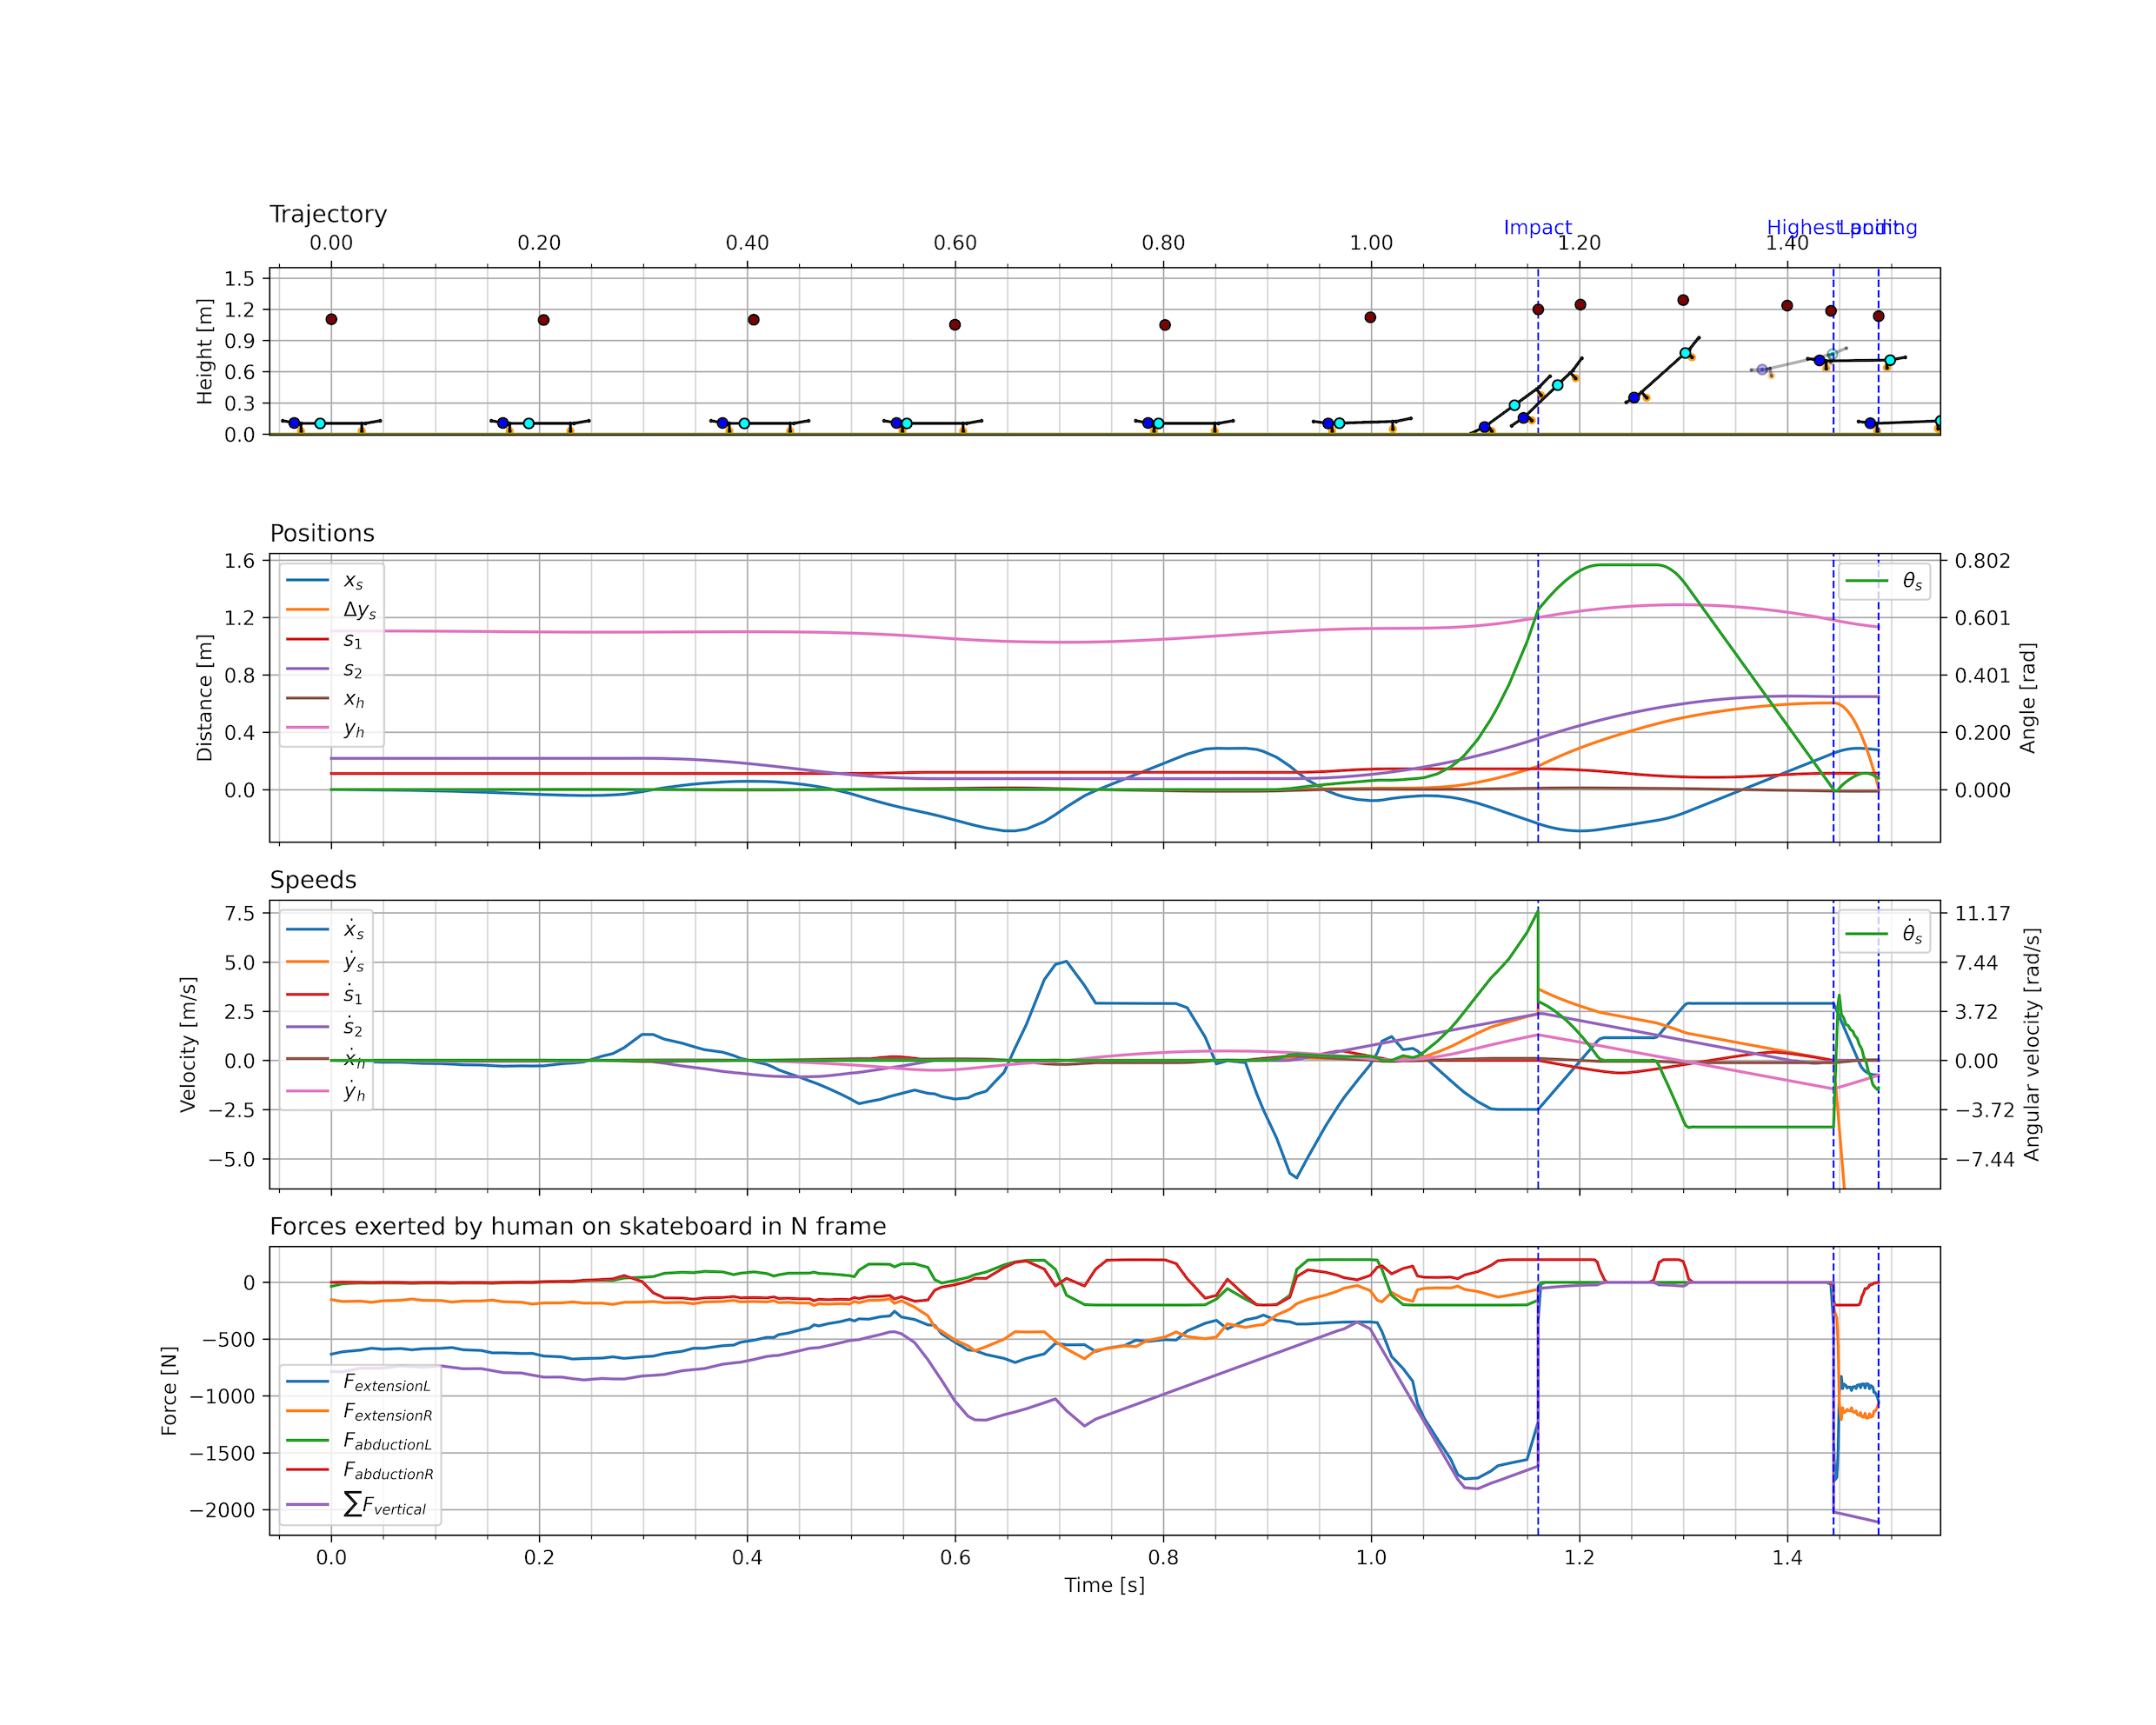
\includegraphics[trim={0cm 0cm 0cm 0cm},clip,width=0.8\textwidth]{figure/Results/data_longboard_init_longer_tail_optdpi600.png}}
    \newline
    \subfloat[All parameters no trucks]{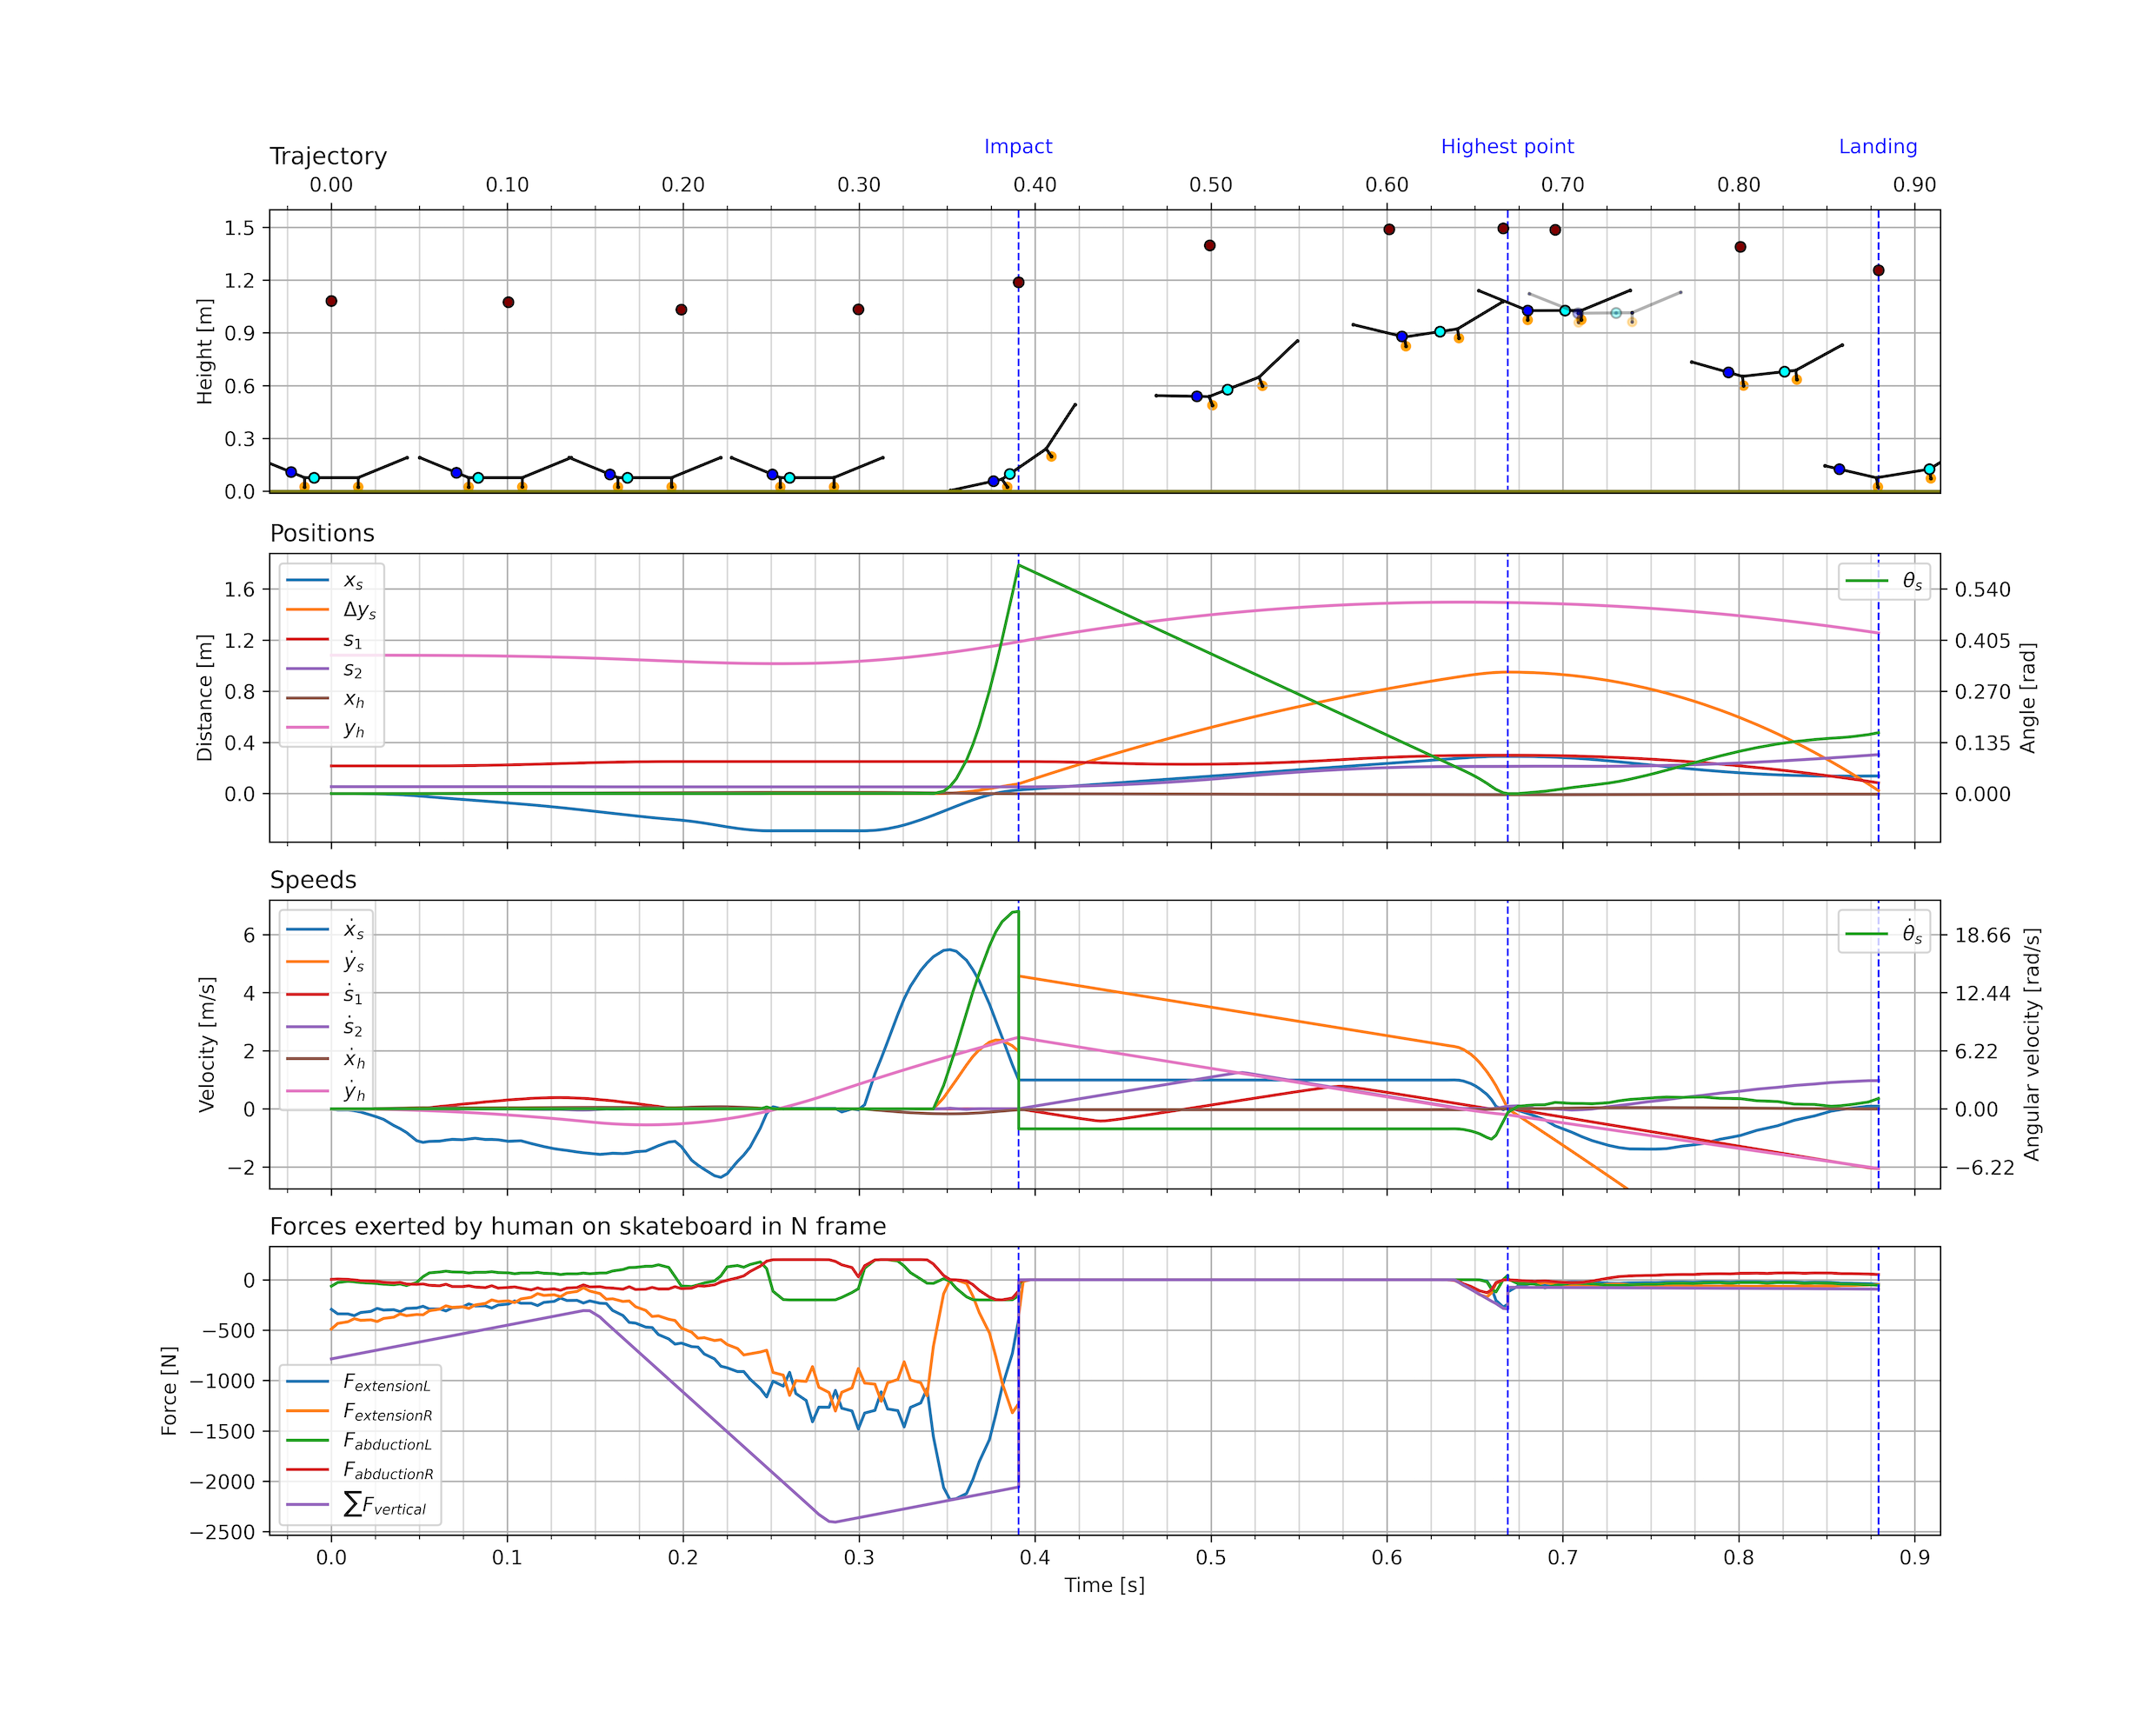
\includegraphics[trim={0cm 0cm 0cm 0cm},clip,width=0.8\textwidth]{figure/Results/data_notrrwdpi600.png}}
    \label{f_longboard}
    \caption{Longboard and `all except trucks' optimization results}
\end{figure*}

\begin{figure*}[b]    
    \subfloat[Plastic]{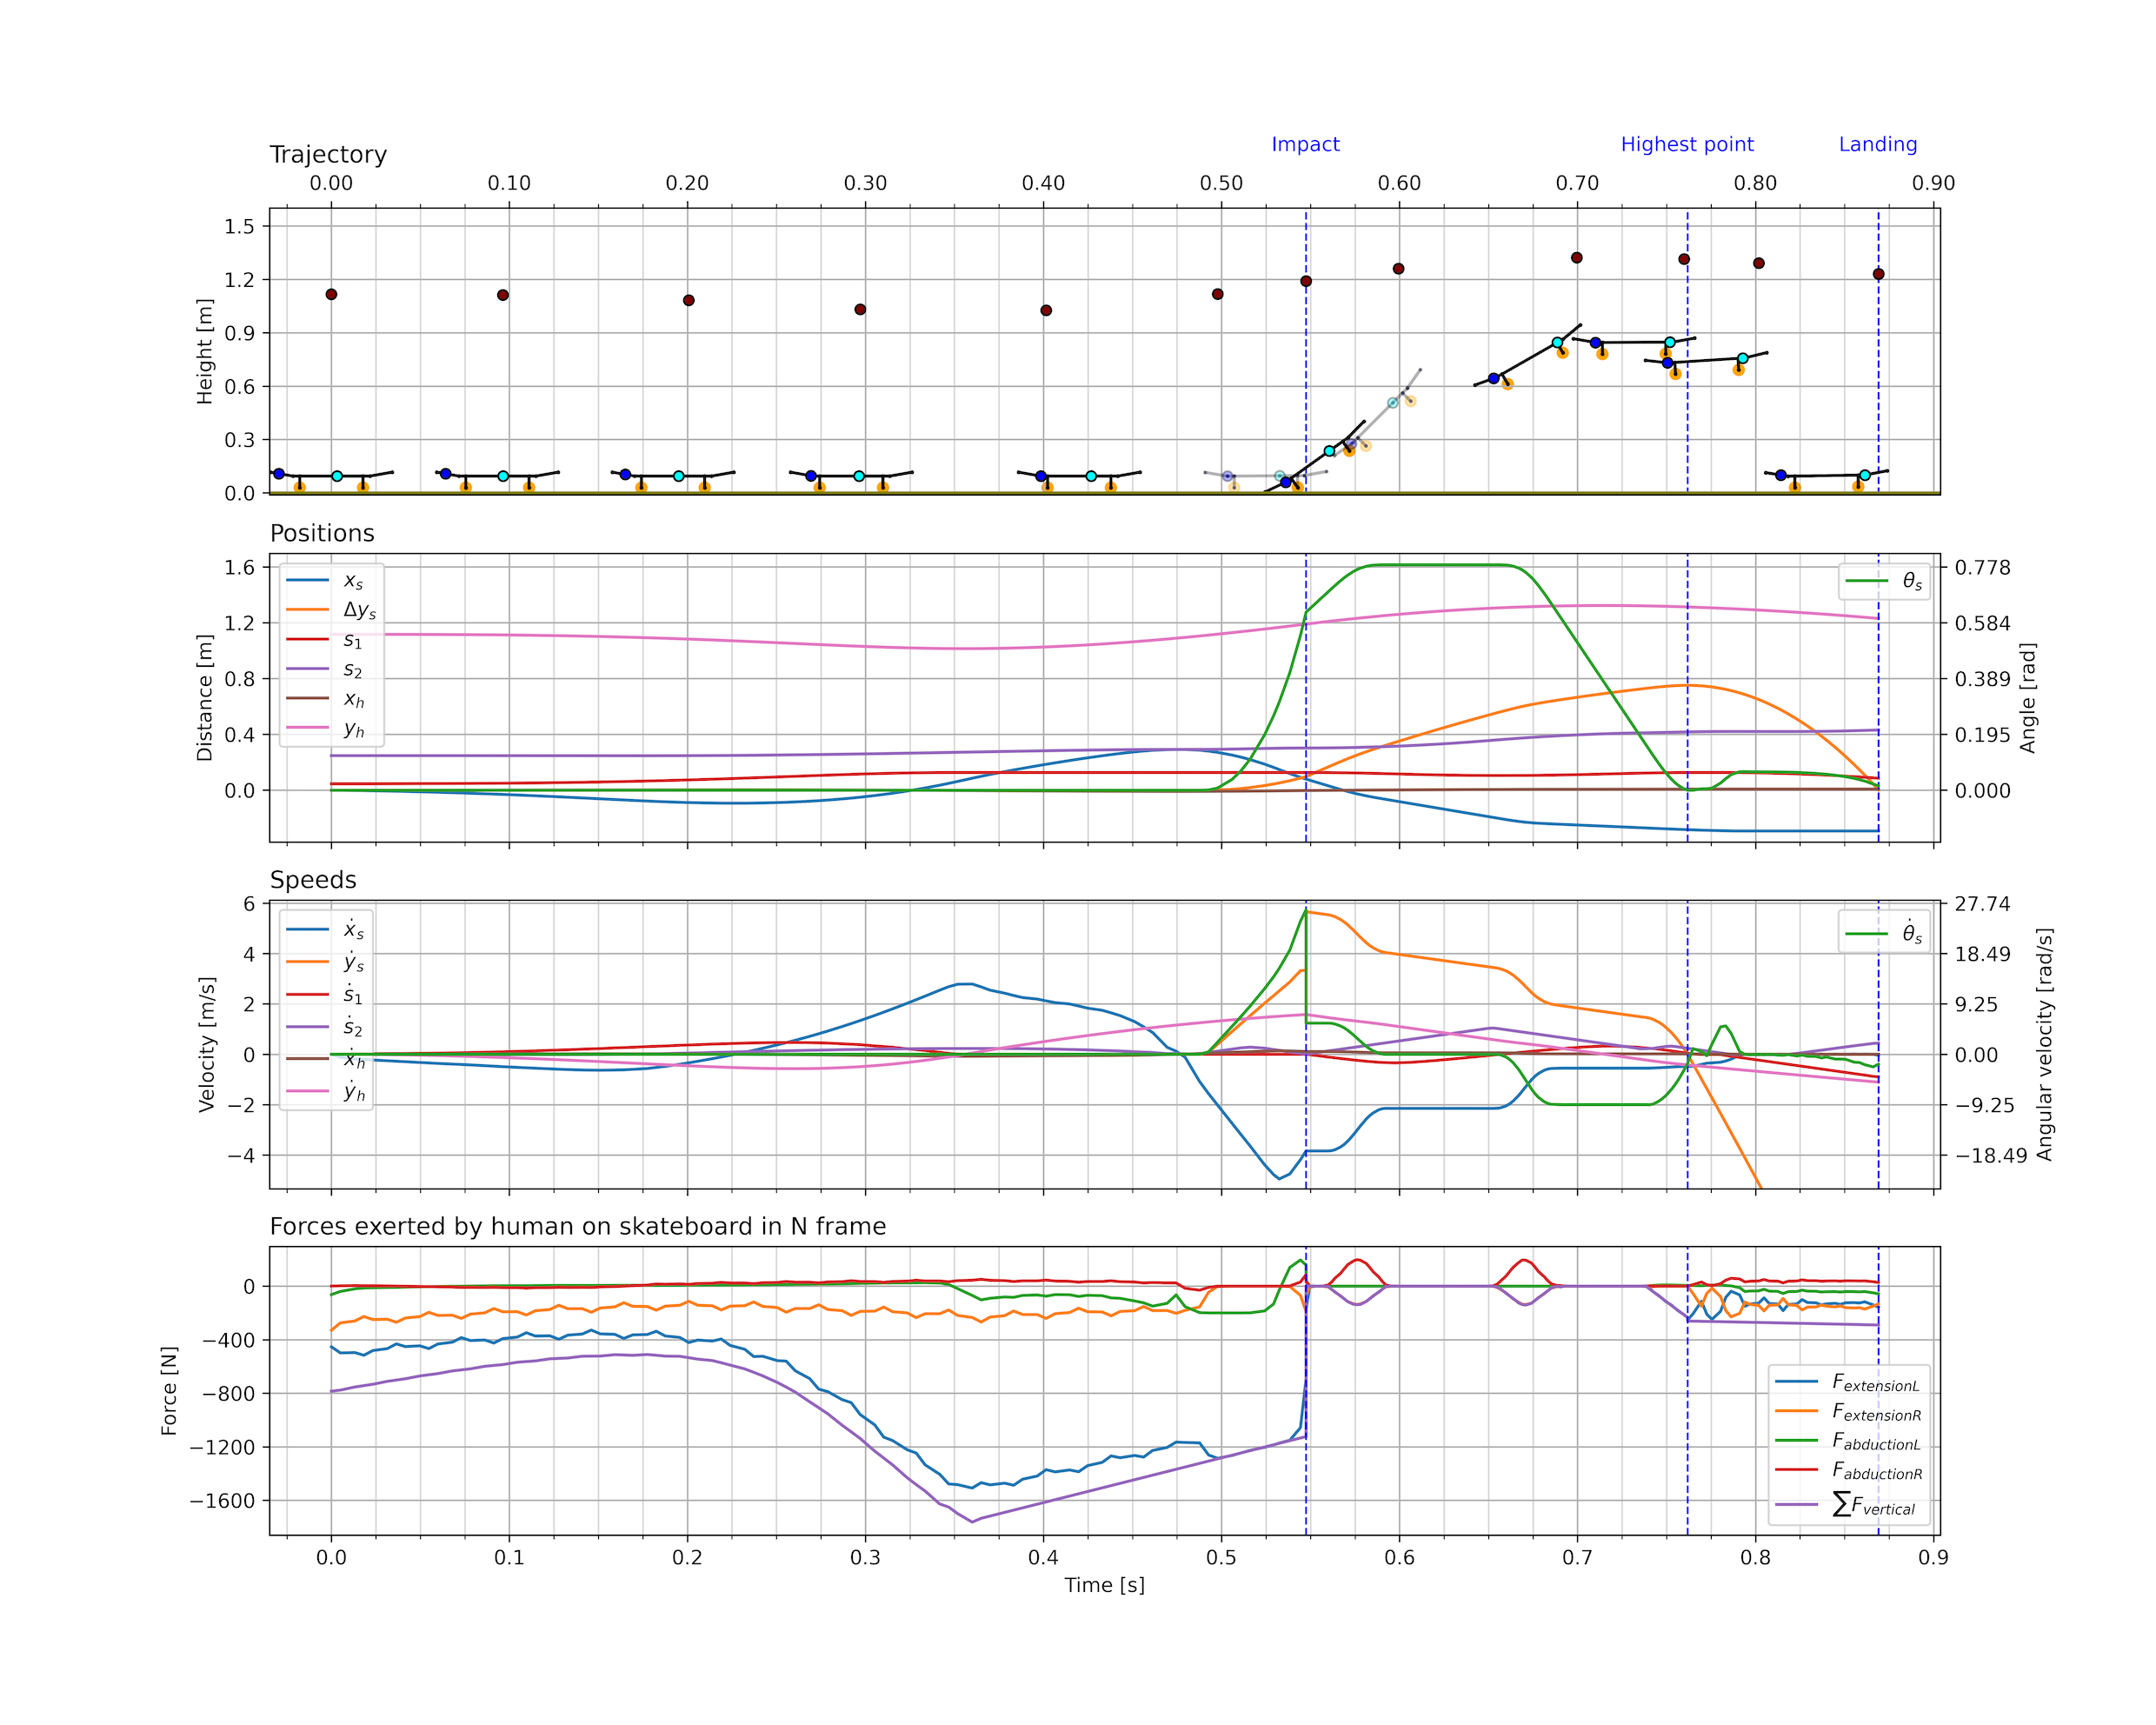
\includegraphics[trim={0cm 0cm 0cm 0cm},clip,width=0.8\textwidth]{figure/Results/data_penny_02dpi600.png}}
    \newline
    \subfloat[Griptape]{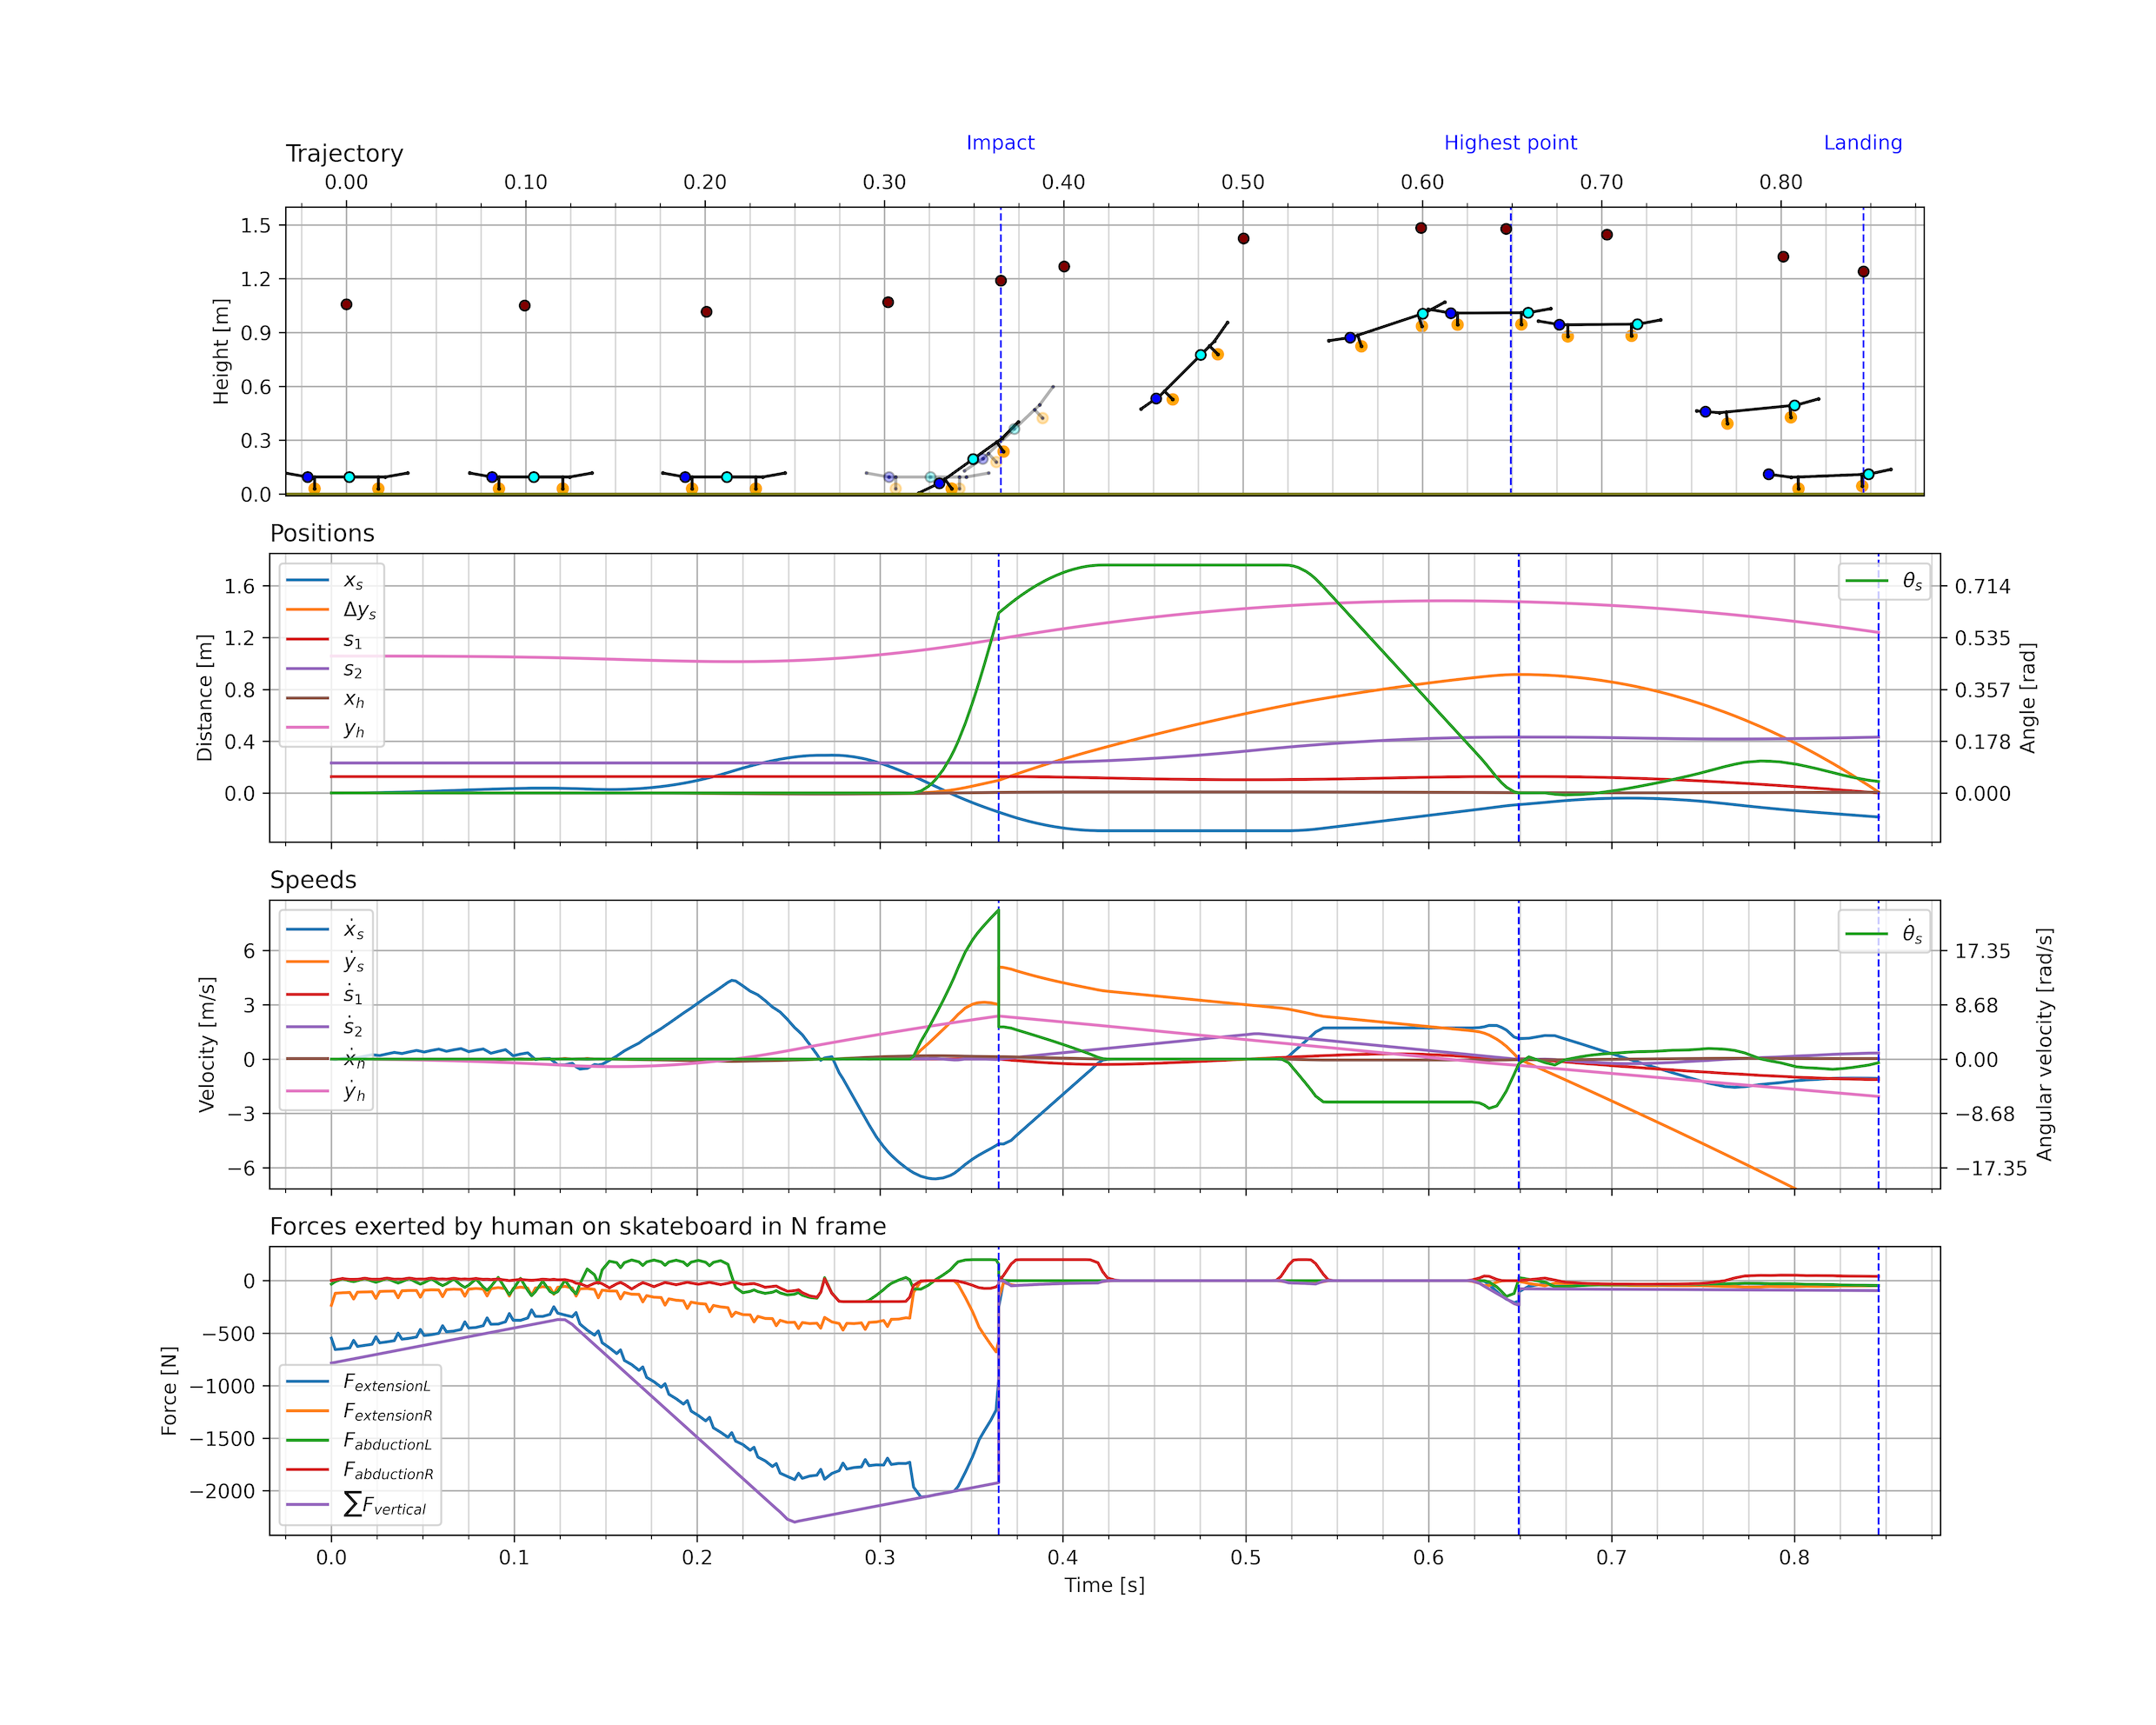
\includegraphics[trim={0cm 0cm 0cm 0cm},clip,width=0.8\textwidth]{figure/Results/data_penny_08dpi600.png}}
    \caption{Penny boards optimization results}    
\end{figure*}

\begin{figure*}[b]    
    \subfloat[Wheel radius]{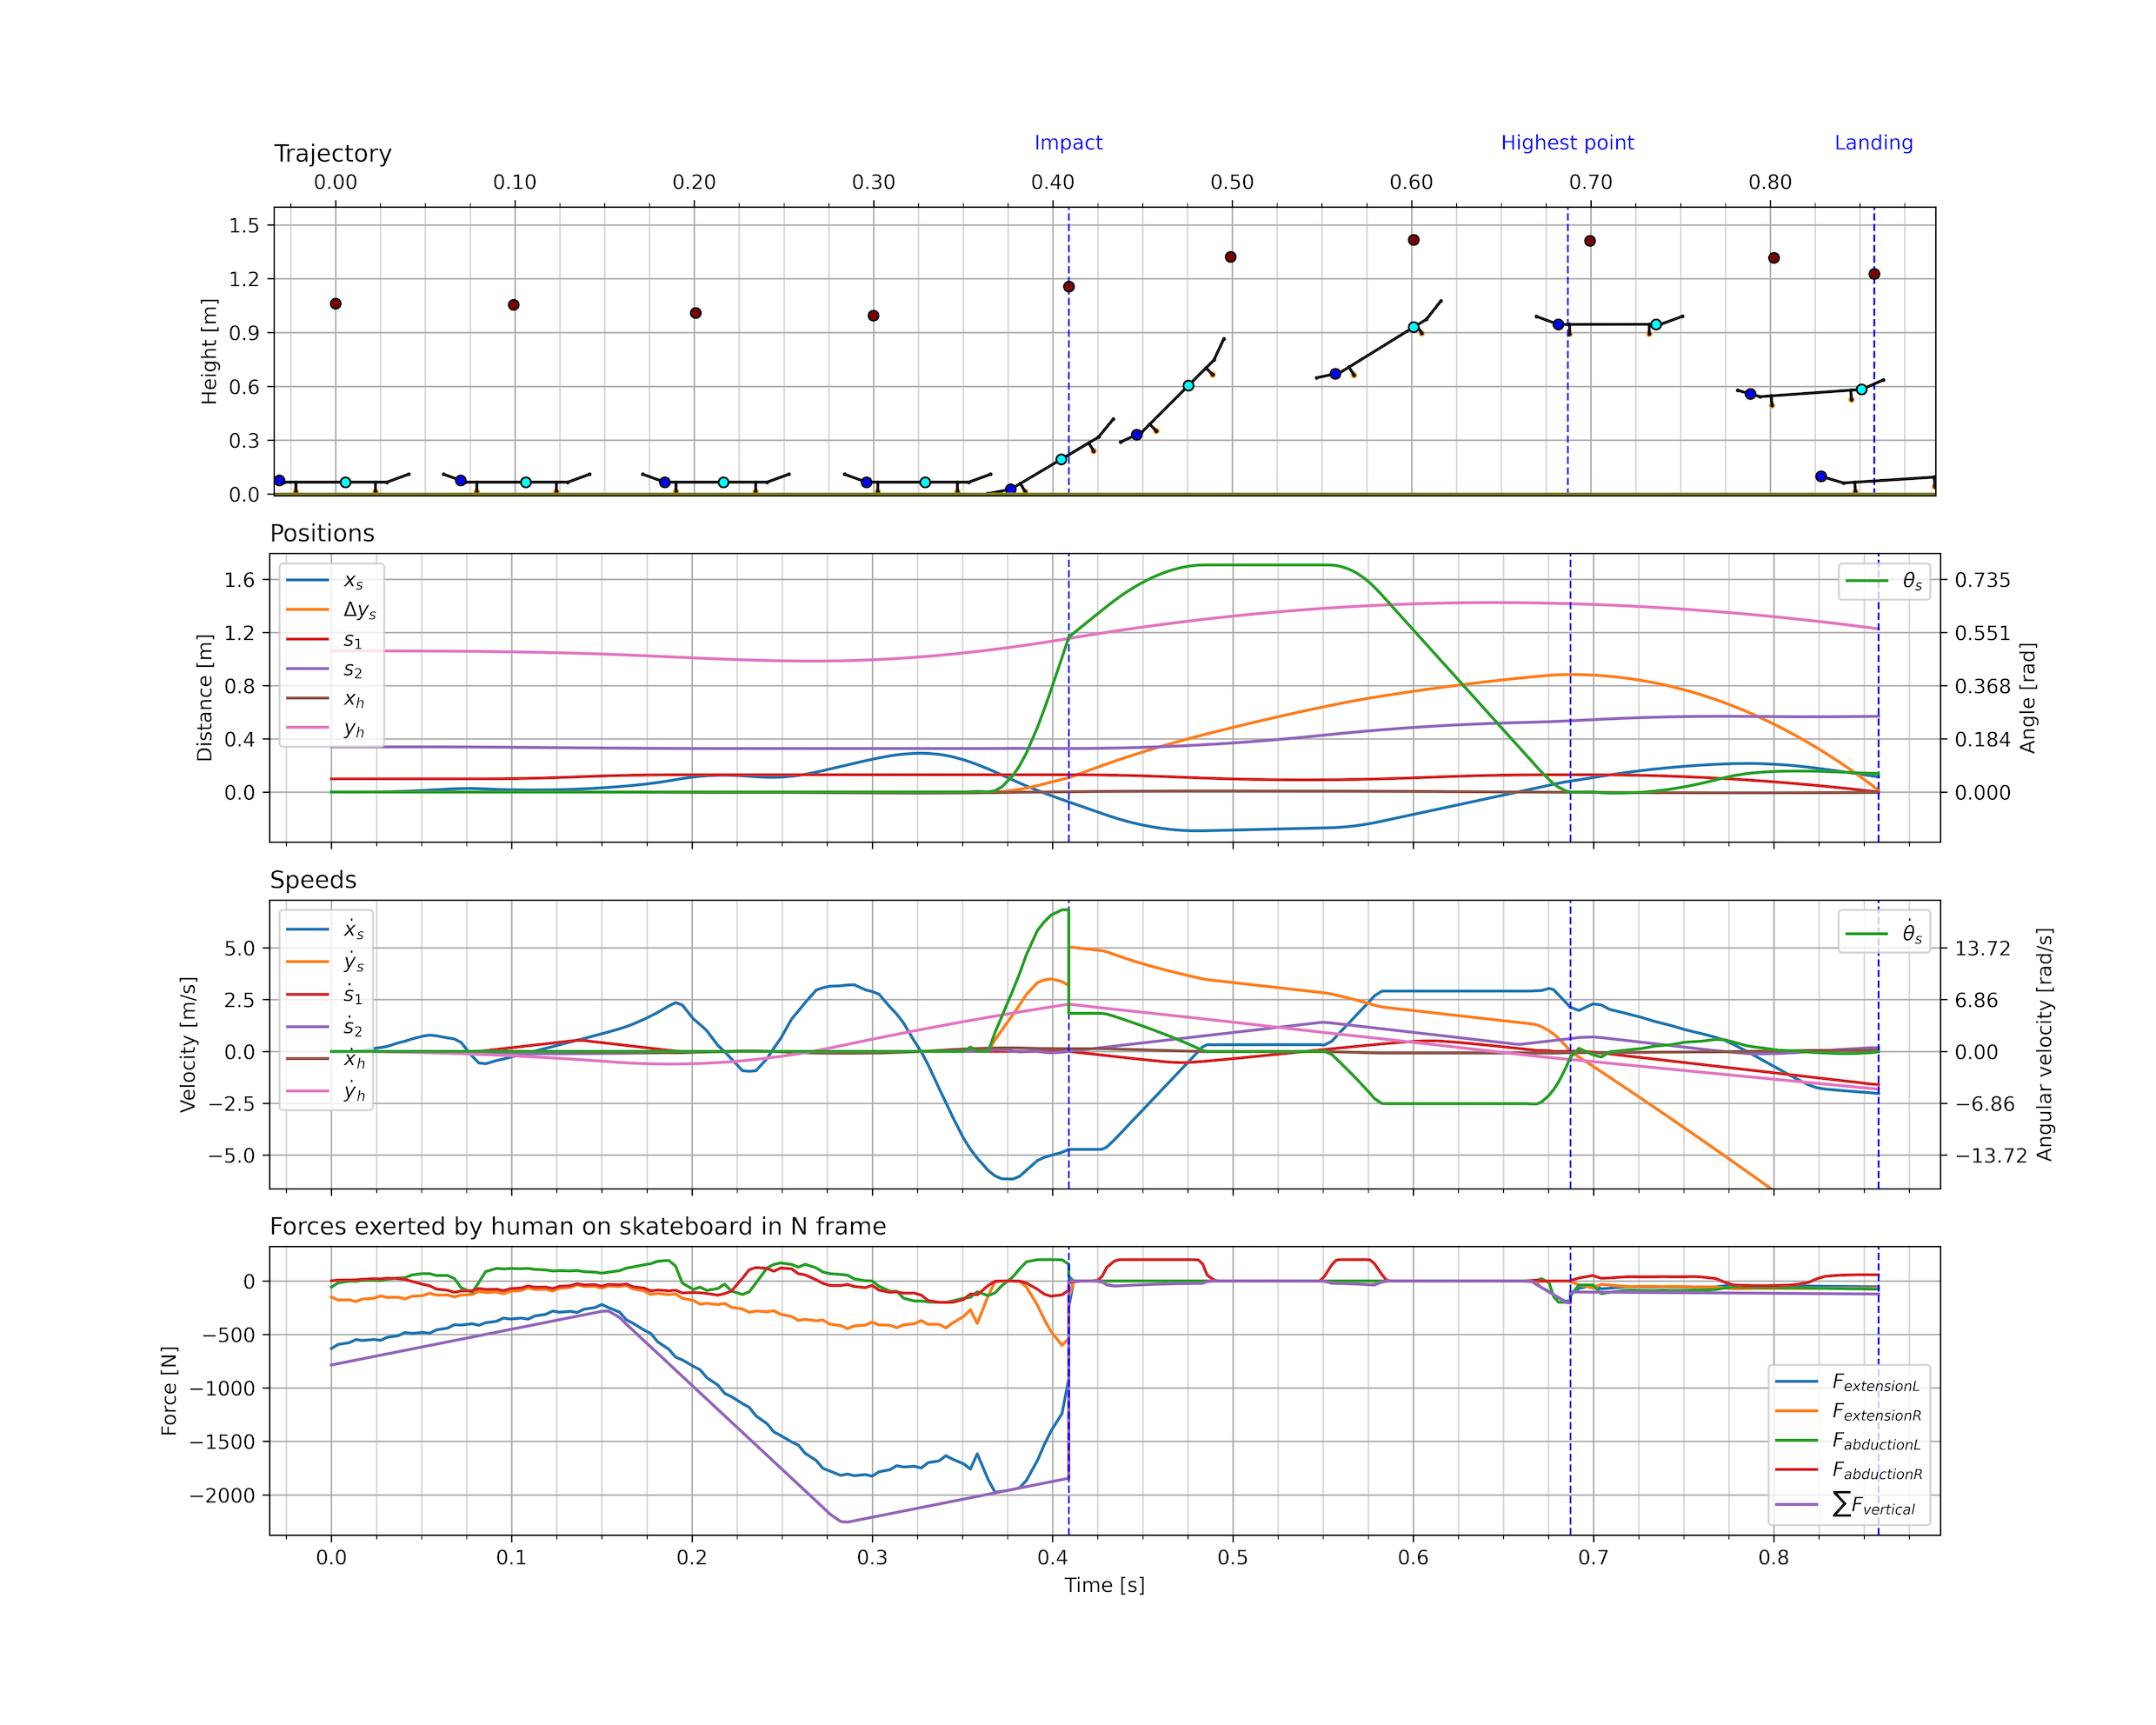
\includegraphics[trim={0cm 0cm 0cm 0cm},clip,width=0.8\textwidth]{figure/Results/data_r_wdpi600.png}}
    \newline
    \subfloat[Truck height]{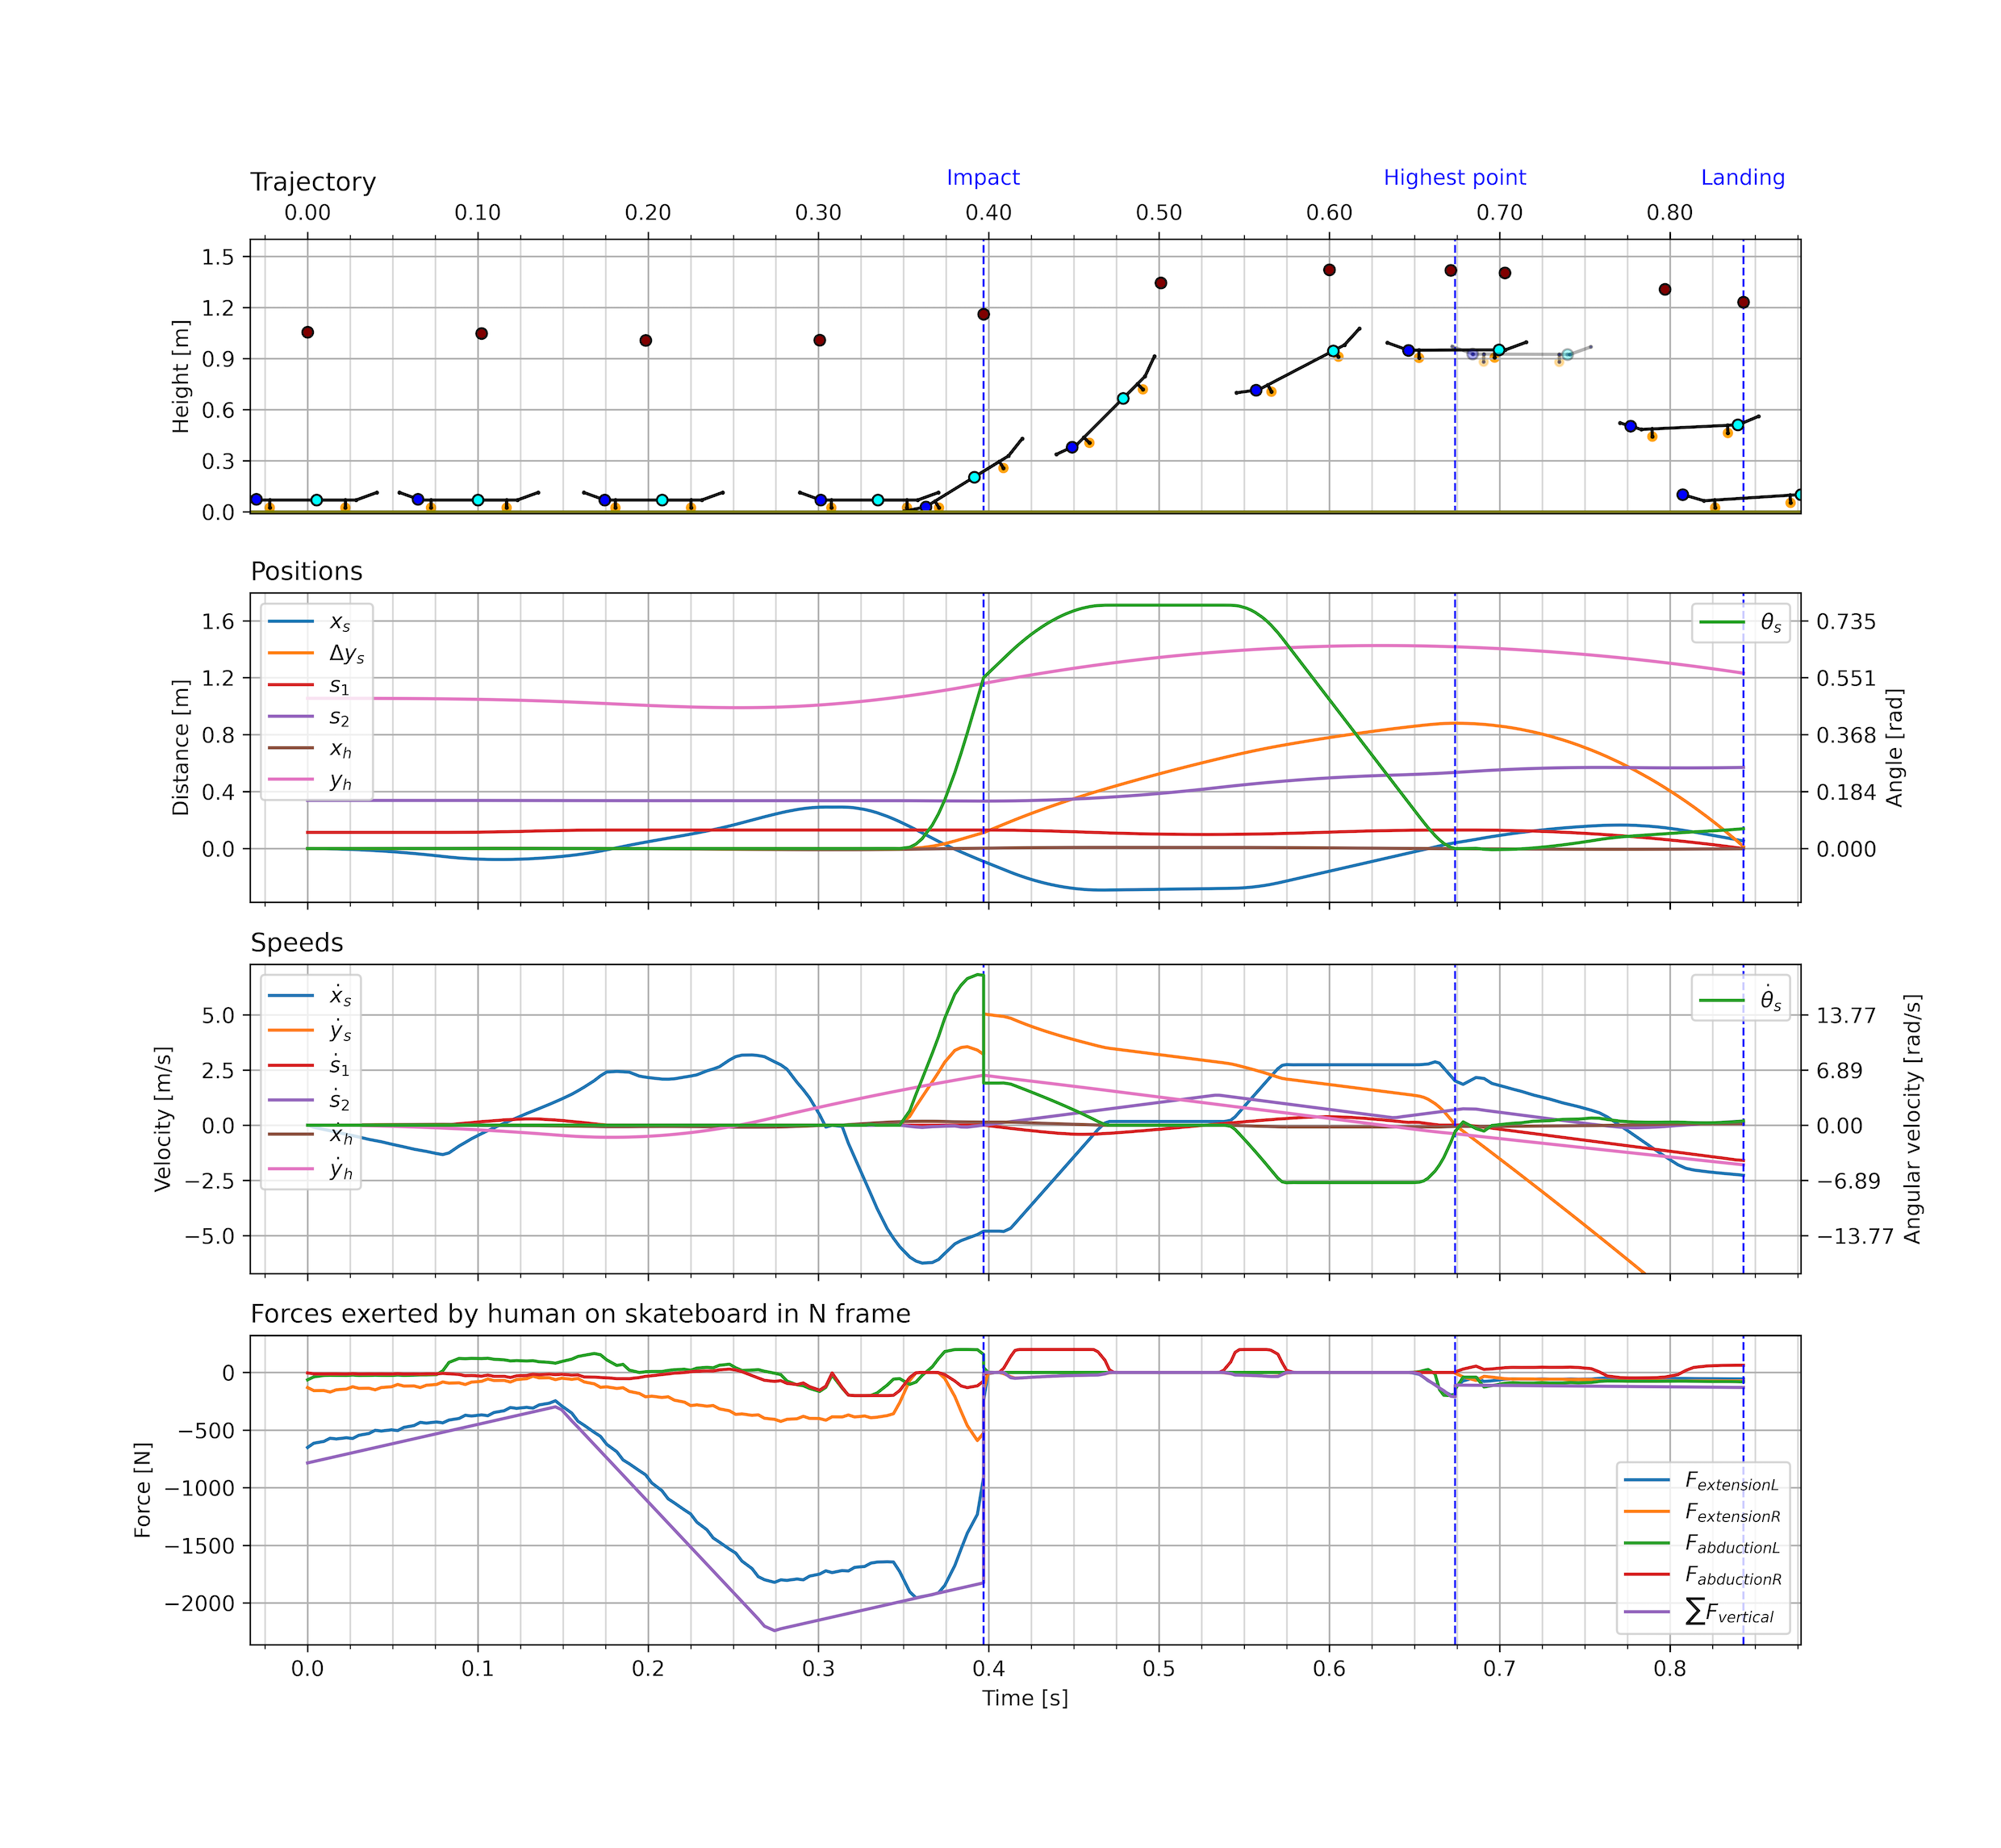
\includegraphics[trim={0cm 0cm 0cm 0cm},clip,width=0.8\textwidth]{figure/Results/data_d_trdpi600.png}}
    \caption{Wheel radius and truck height optimization results}    
\end{figure*}

% \begin{figure*}[b]    
%     \subfloat[Wheel radius]{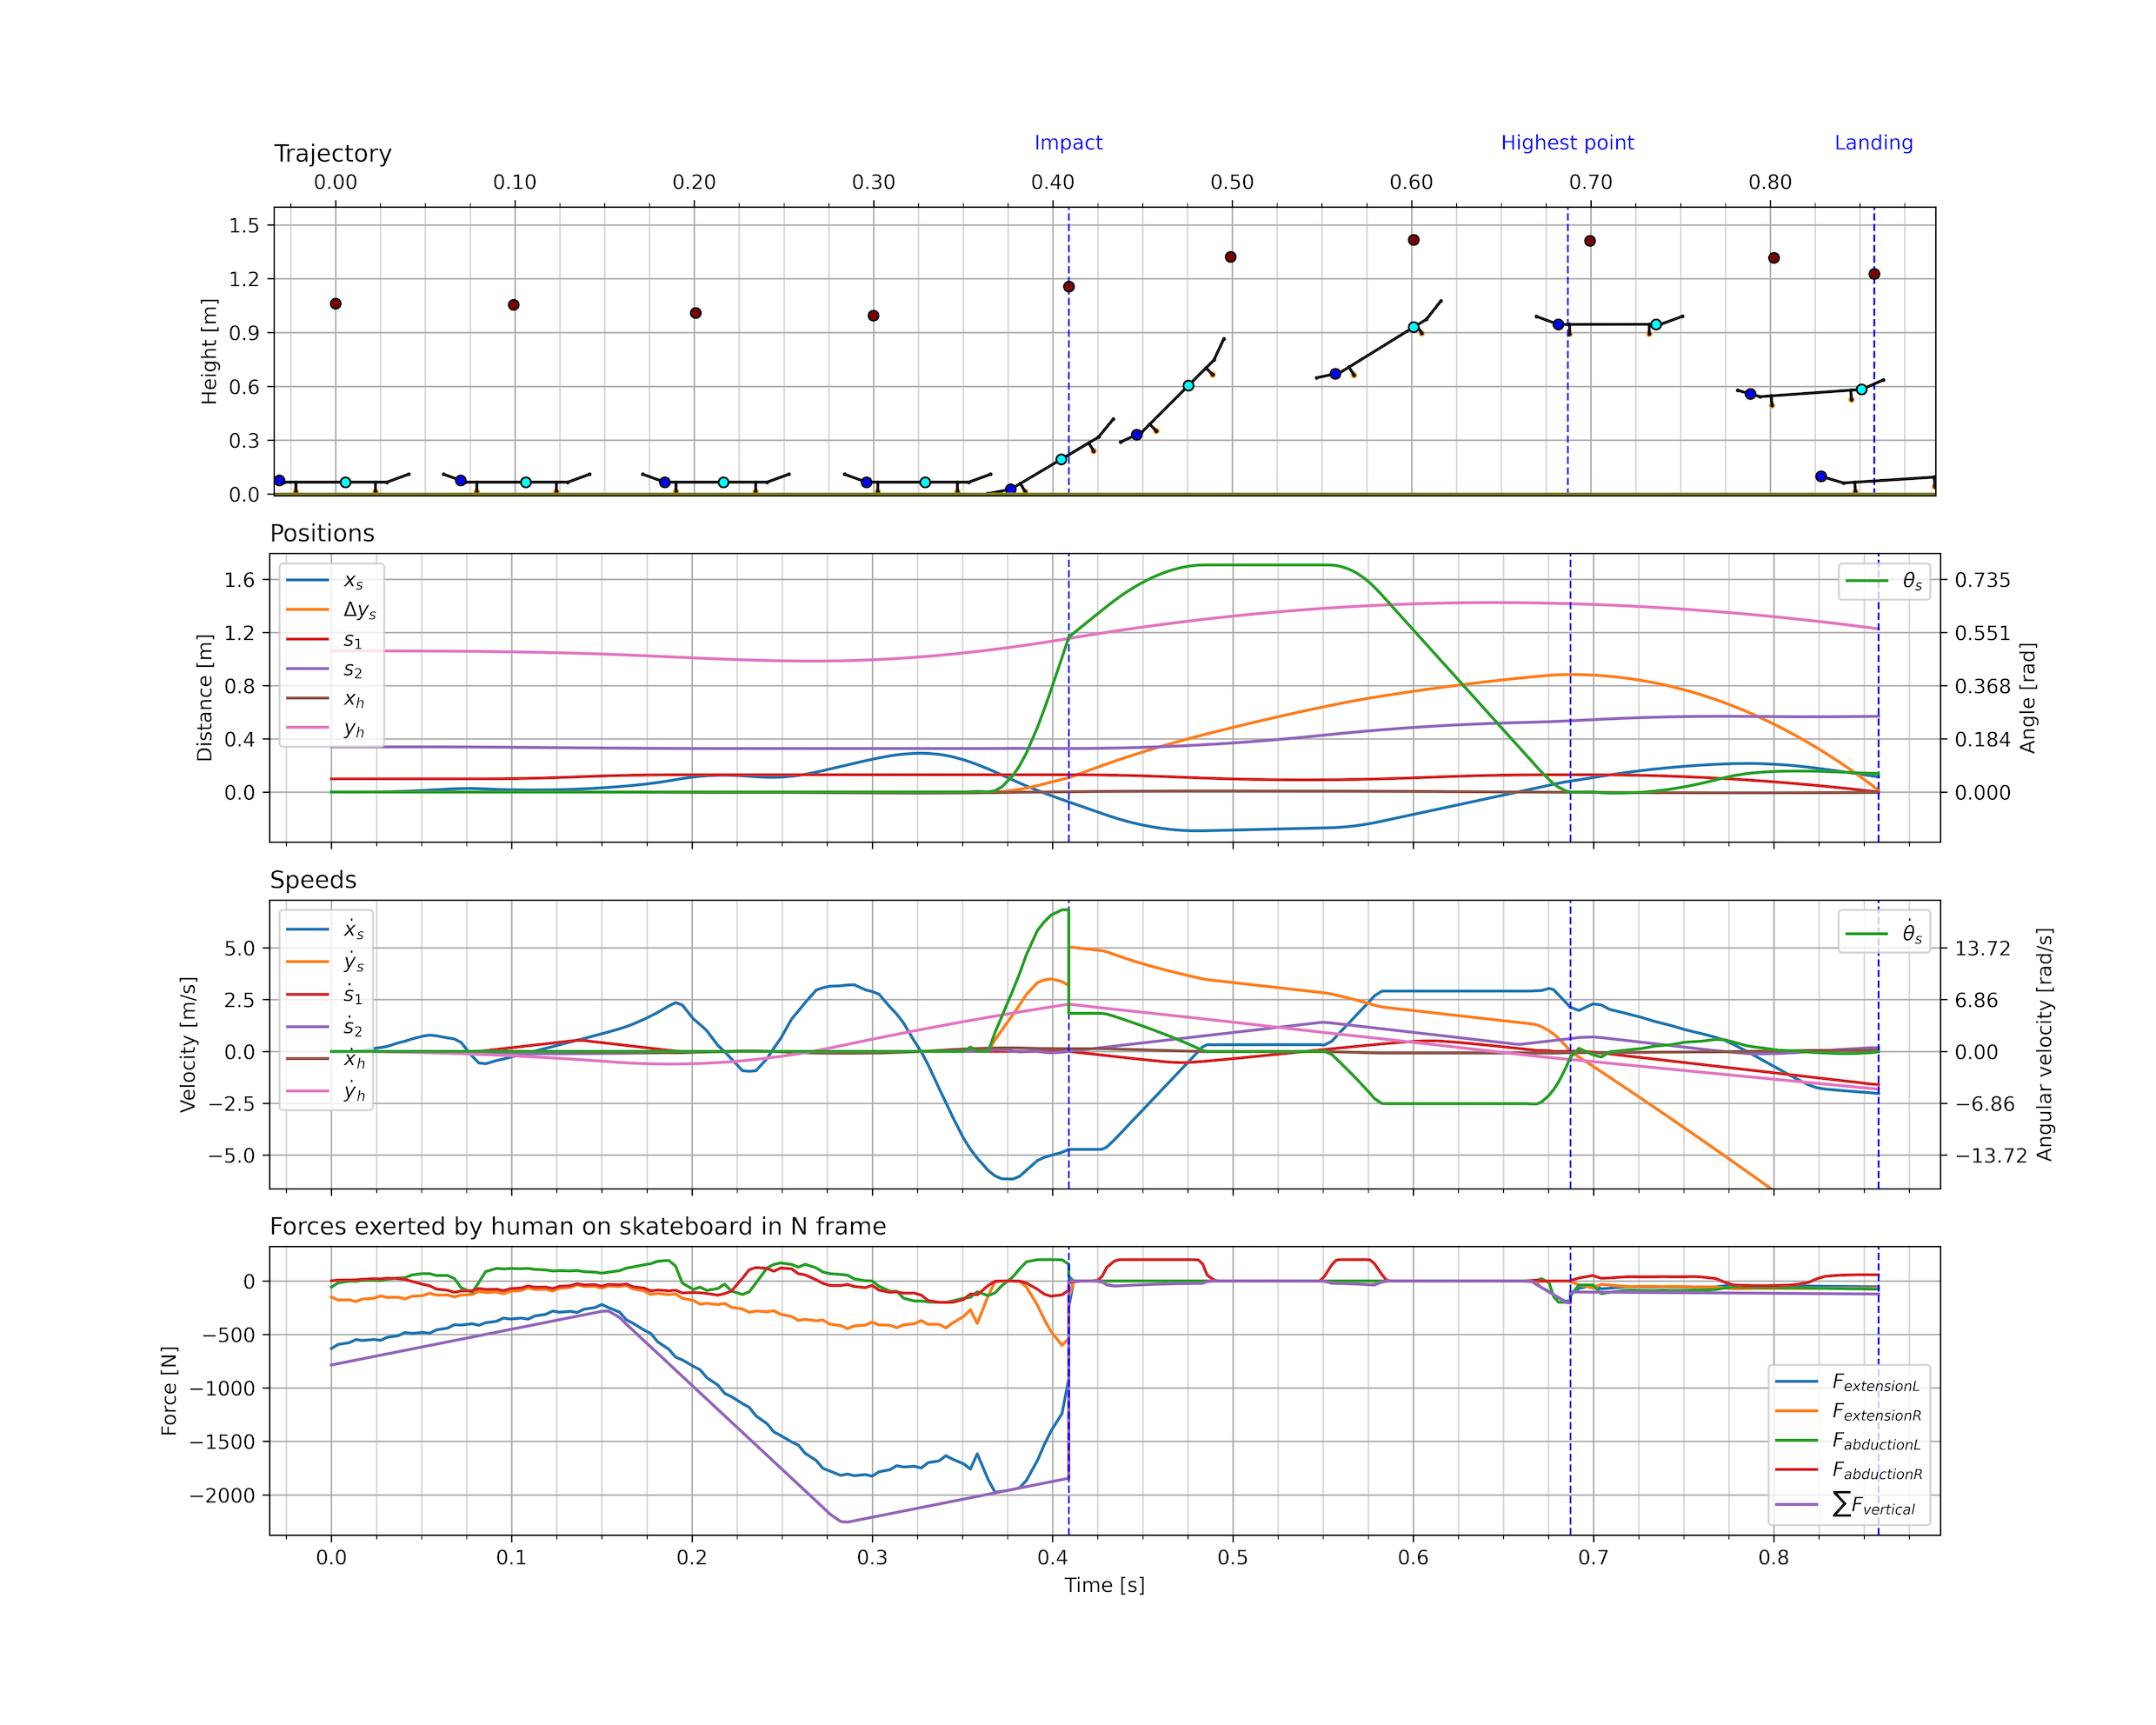
\includegraphics[trim={0cm 0cm 0cm 0cm},clip,width=0.8\textwidth]{figure/Results/data_r_wdpi600.png}}
%     \newline
%     \subfloat[Truck height]{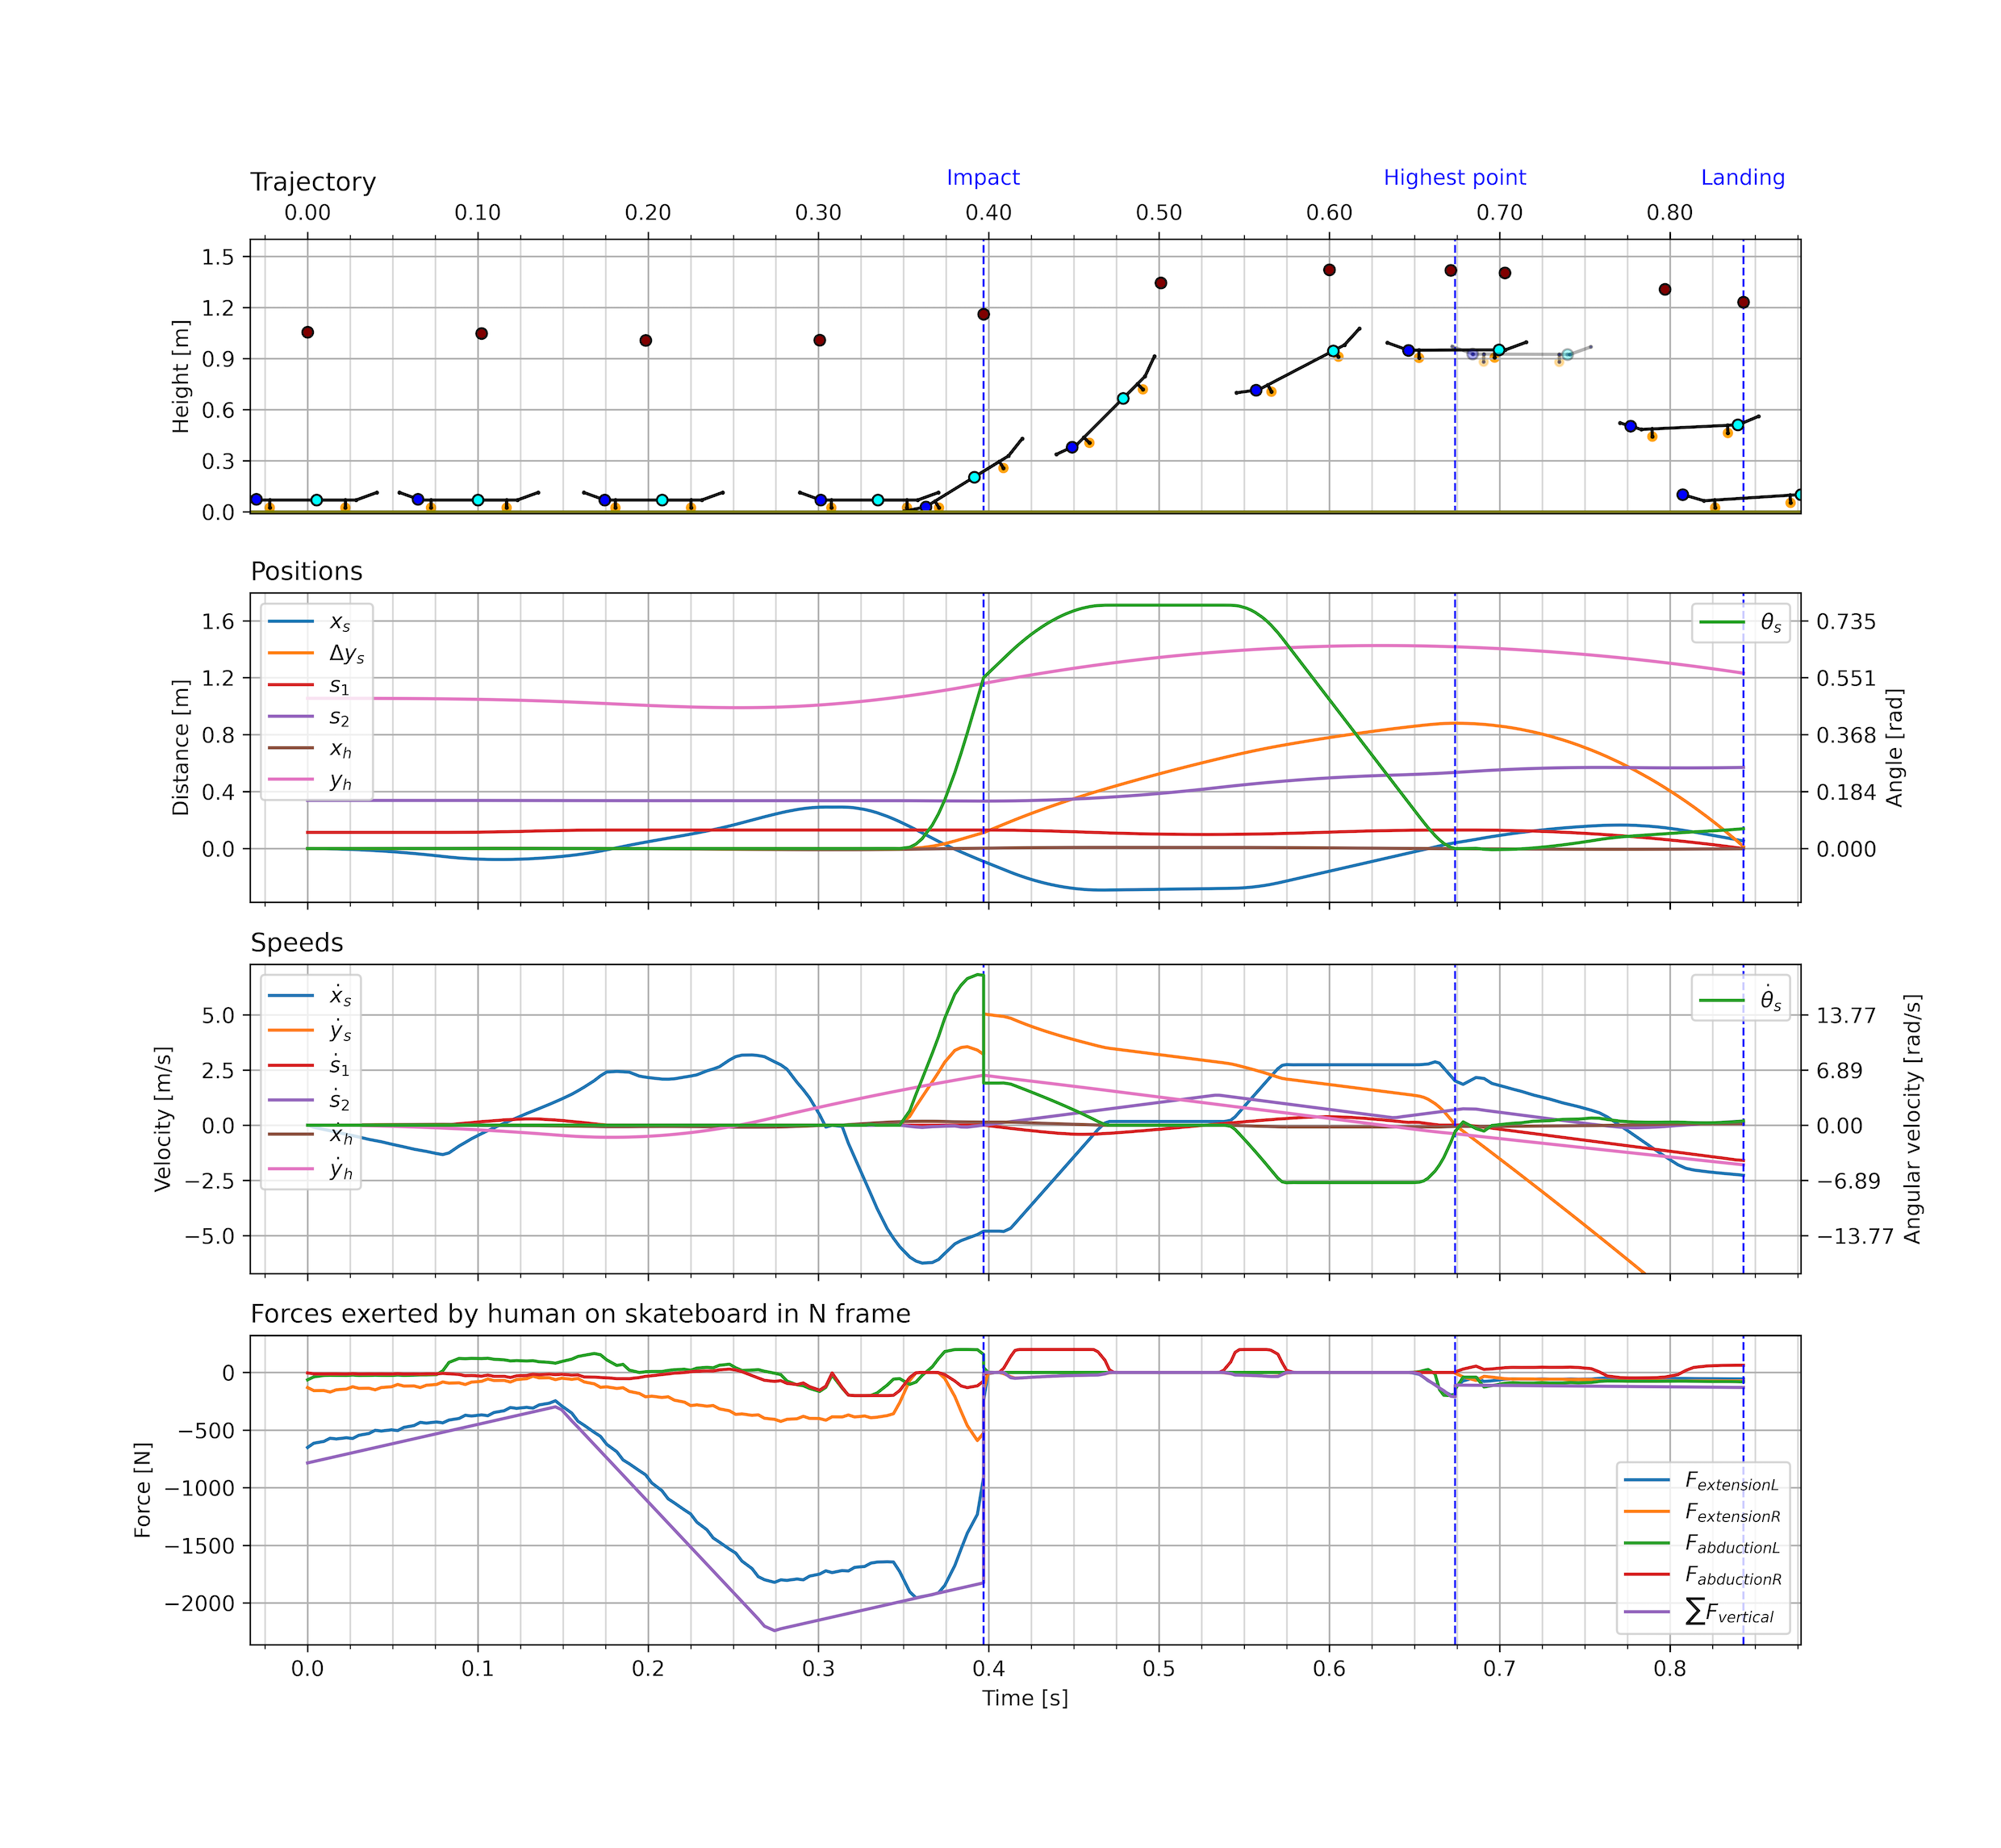
\includegraphics[trim={0cm 0cm 0cm 0cm},clip,width=0.8\textwidth]{figure/Results/data_d_trdpi600.png}}
%     \caption{Single parameter optimization}    
% \end{figure*}

\begin{figure*}[b]    
    \subfloat[Deck length]{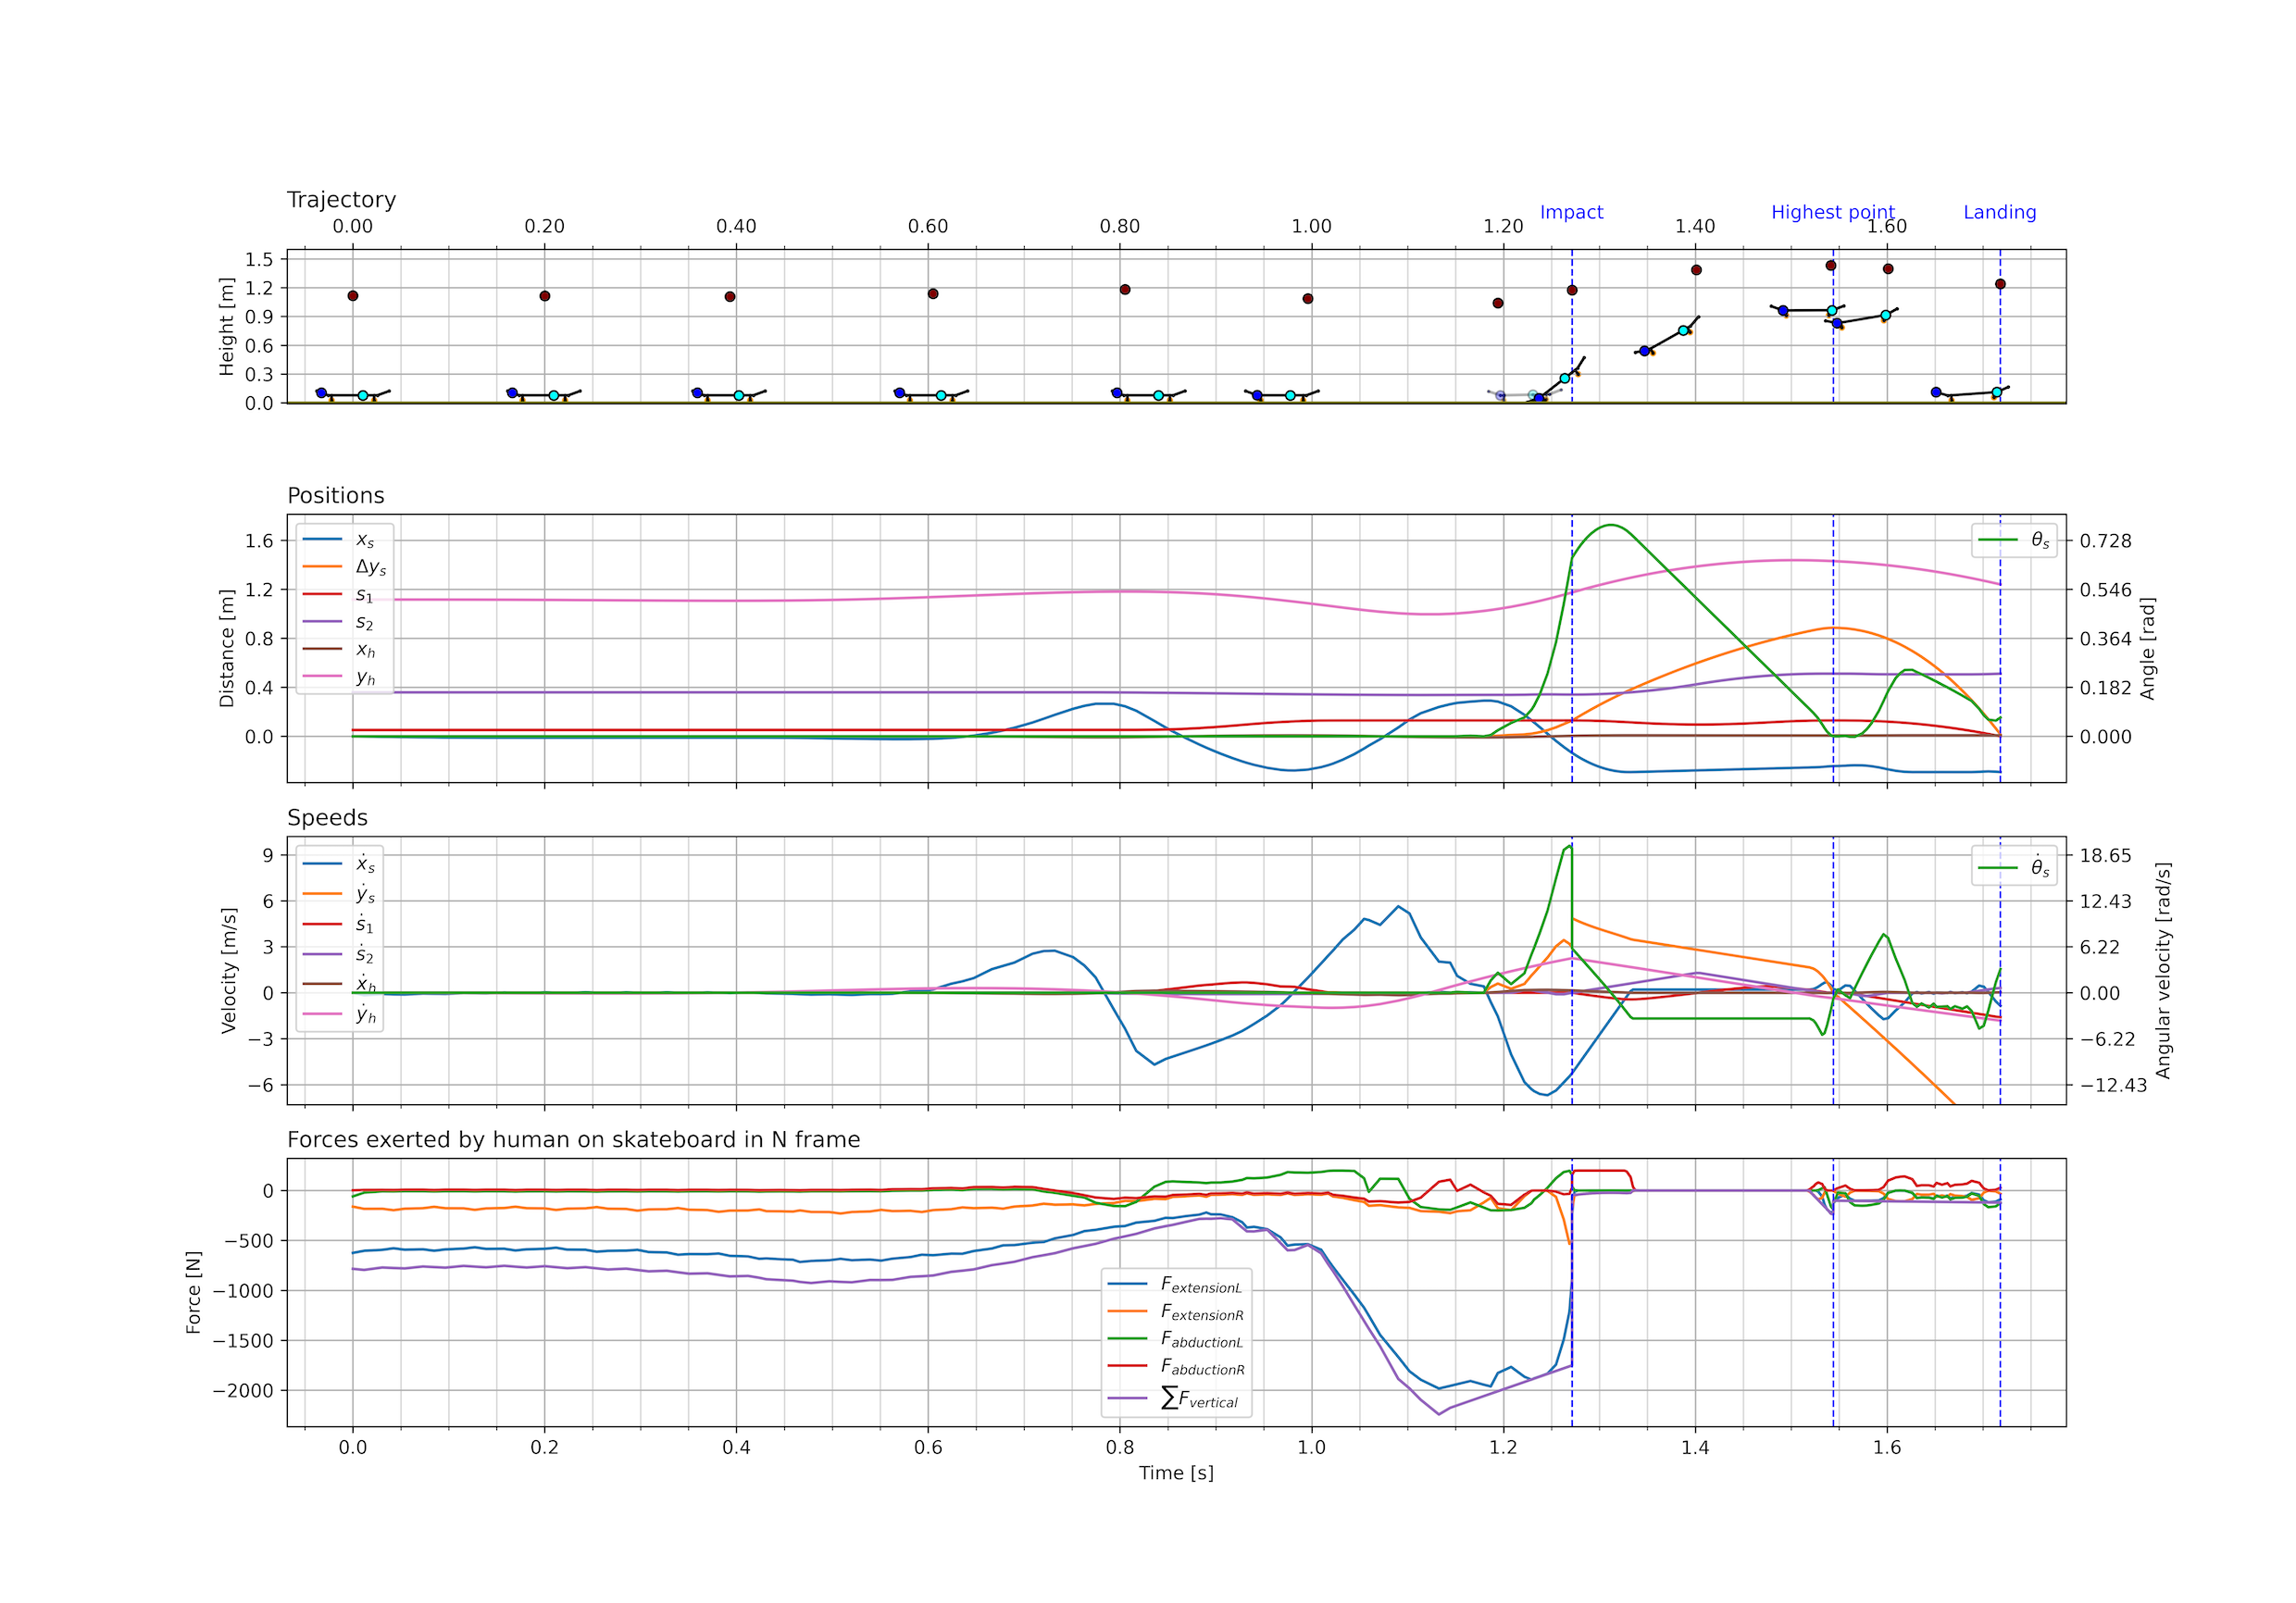
\includegraphics[trim={0cm 0cm 0cm 0cm},clip,width=0.8\textwidth]{figure/Results/data_l_fdpi600.png}}
    \newline
    \subfloat[Tail length]{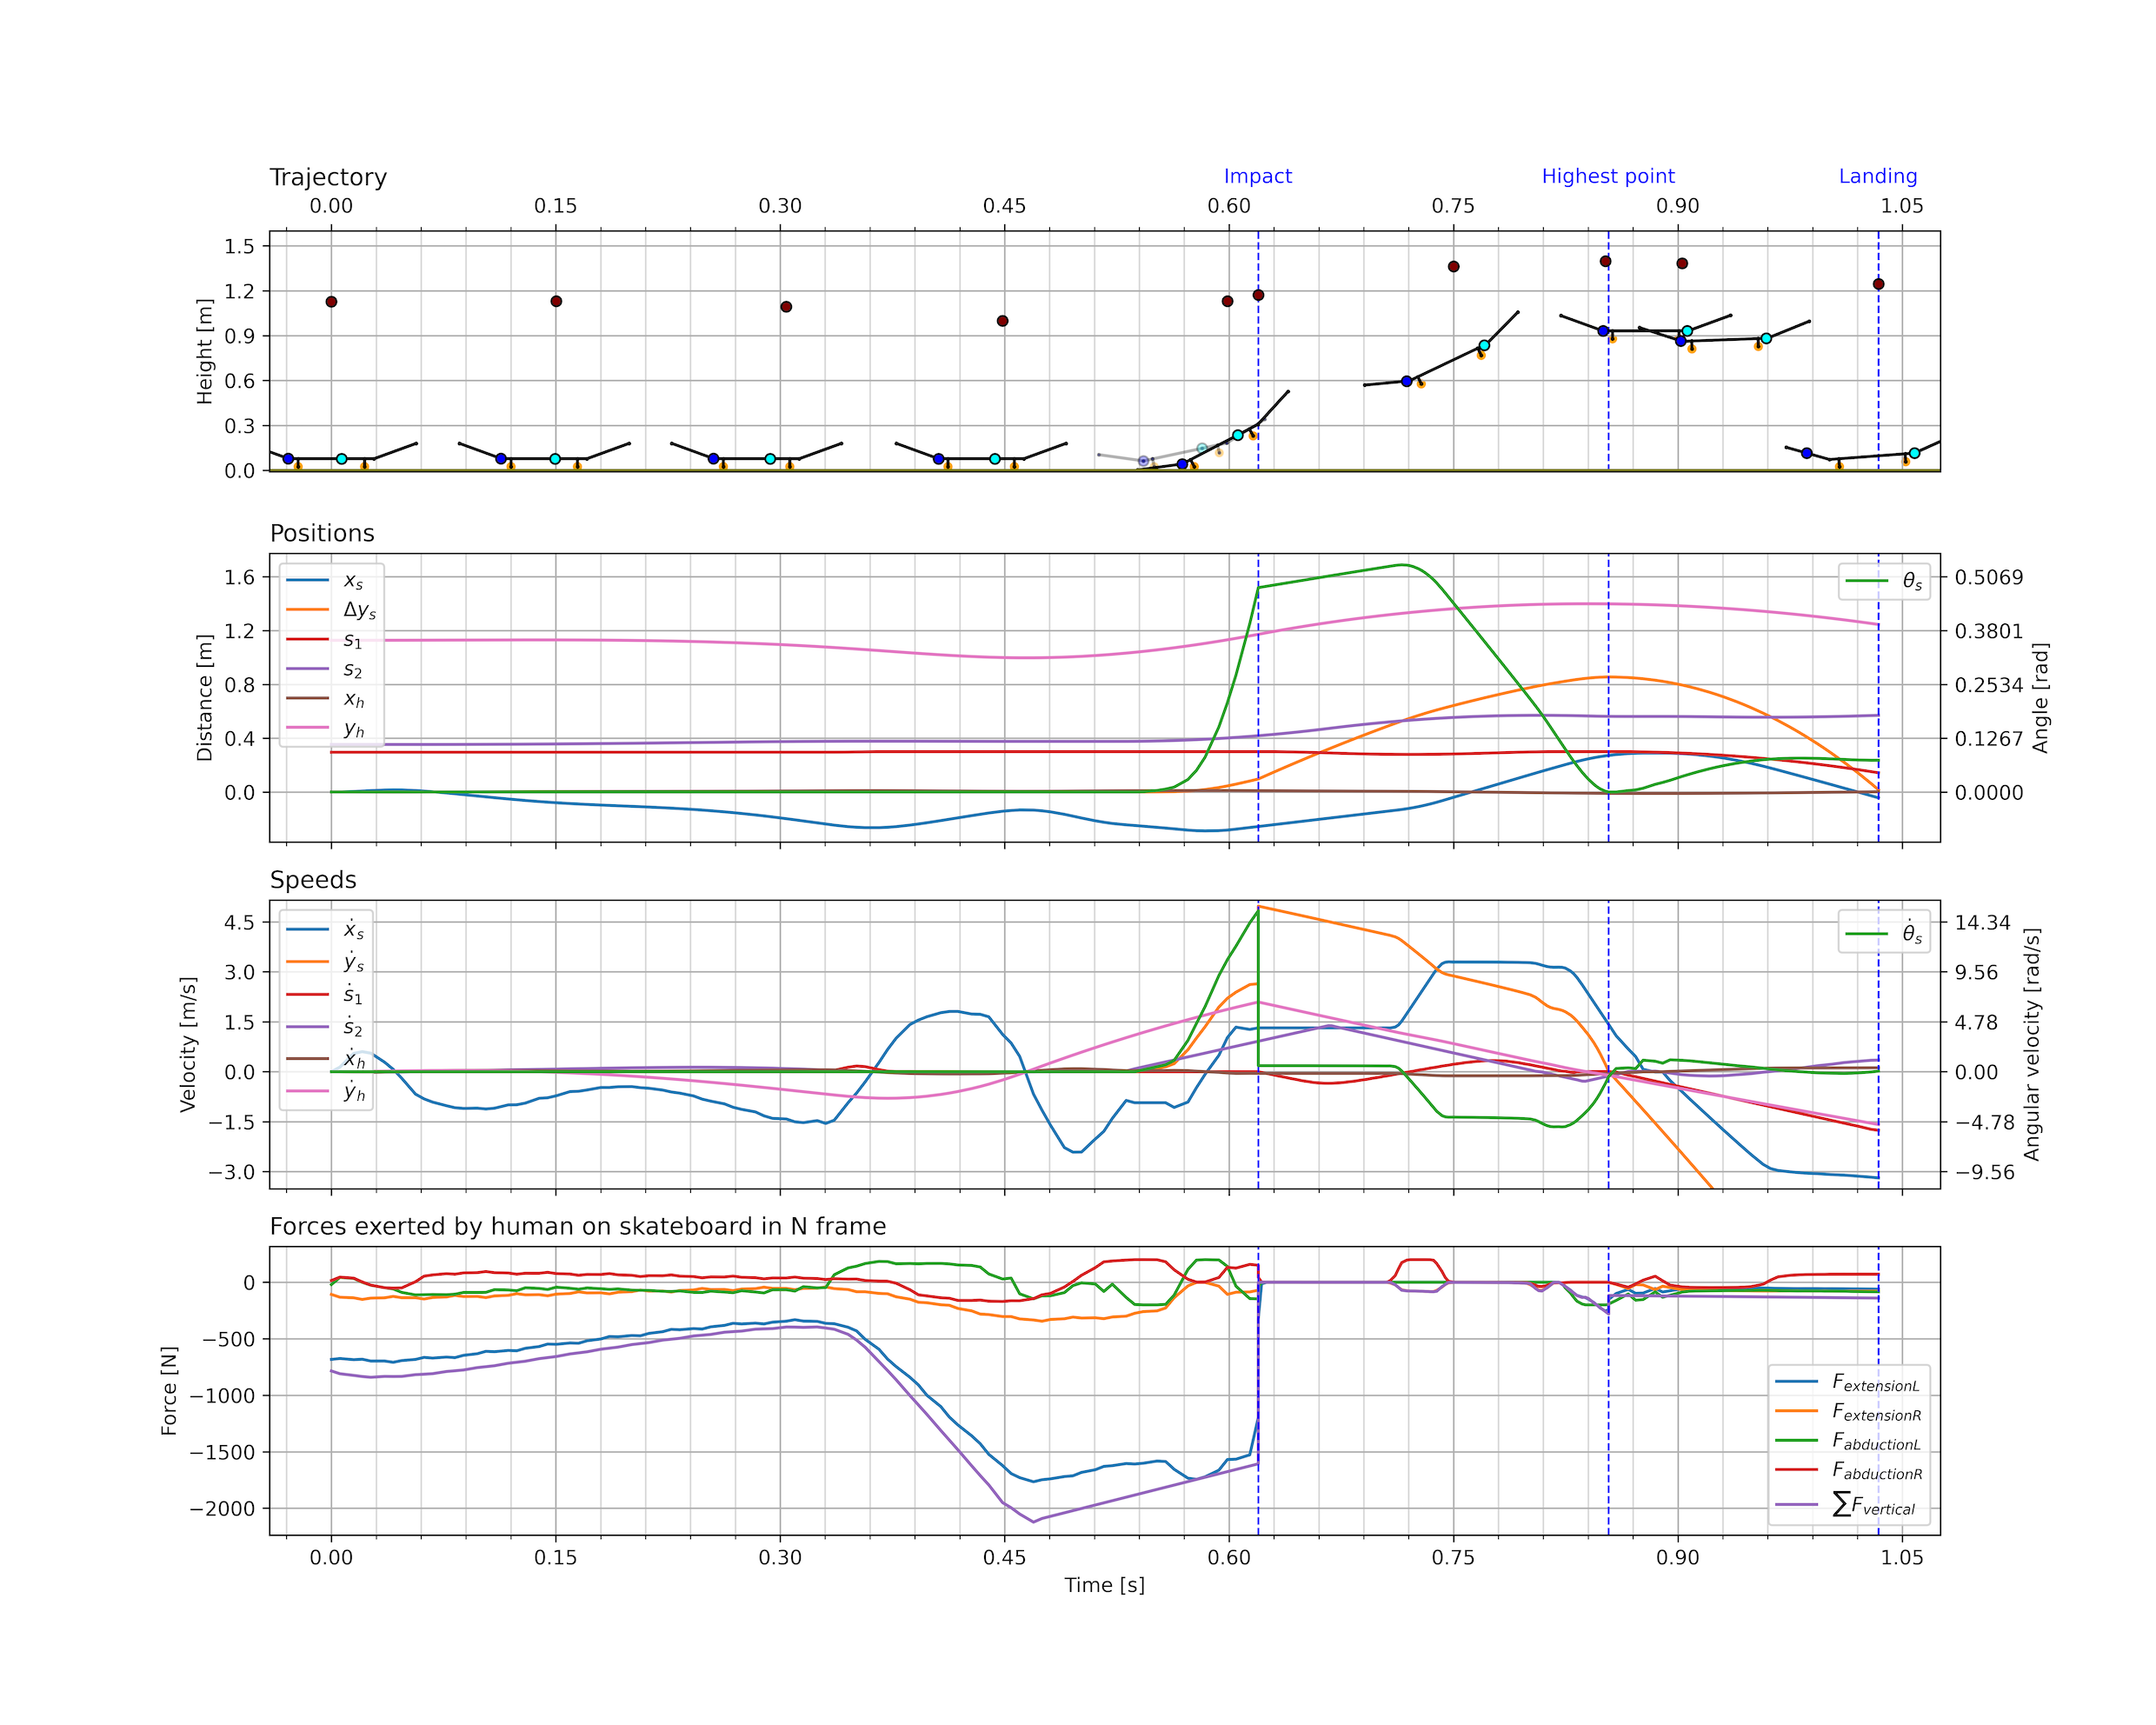
\includegraphics[trim={0cm 0cm 0cm 0cm},clip,width=0.8\textwidth]{figure/Results/data_l_tdpi600.png}}
    \caption{Deck length and tail length optimization results}    
\end{figure*}

\begin{figure*}[b]    
    \subfloat[Tail inclination]{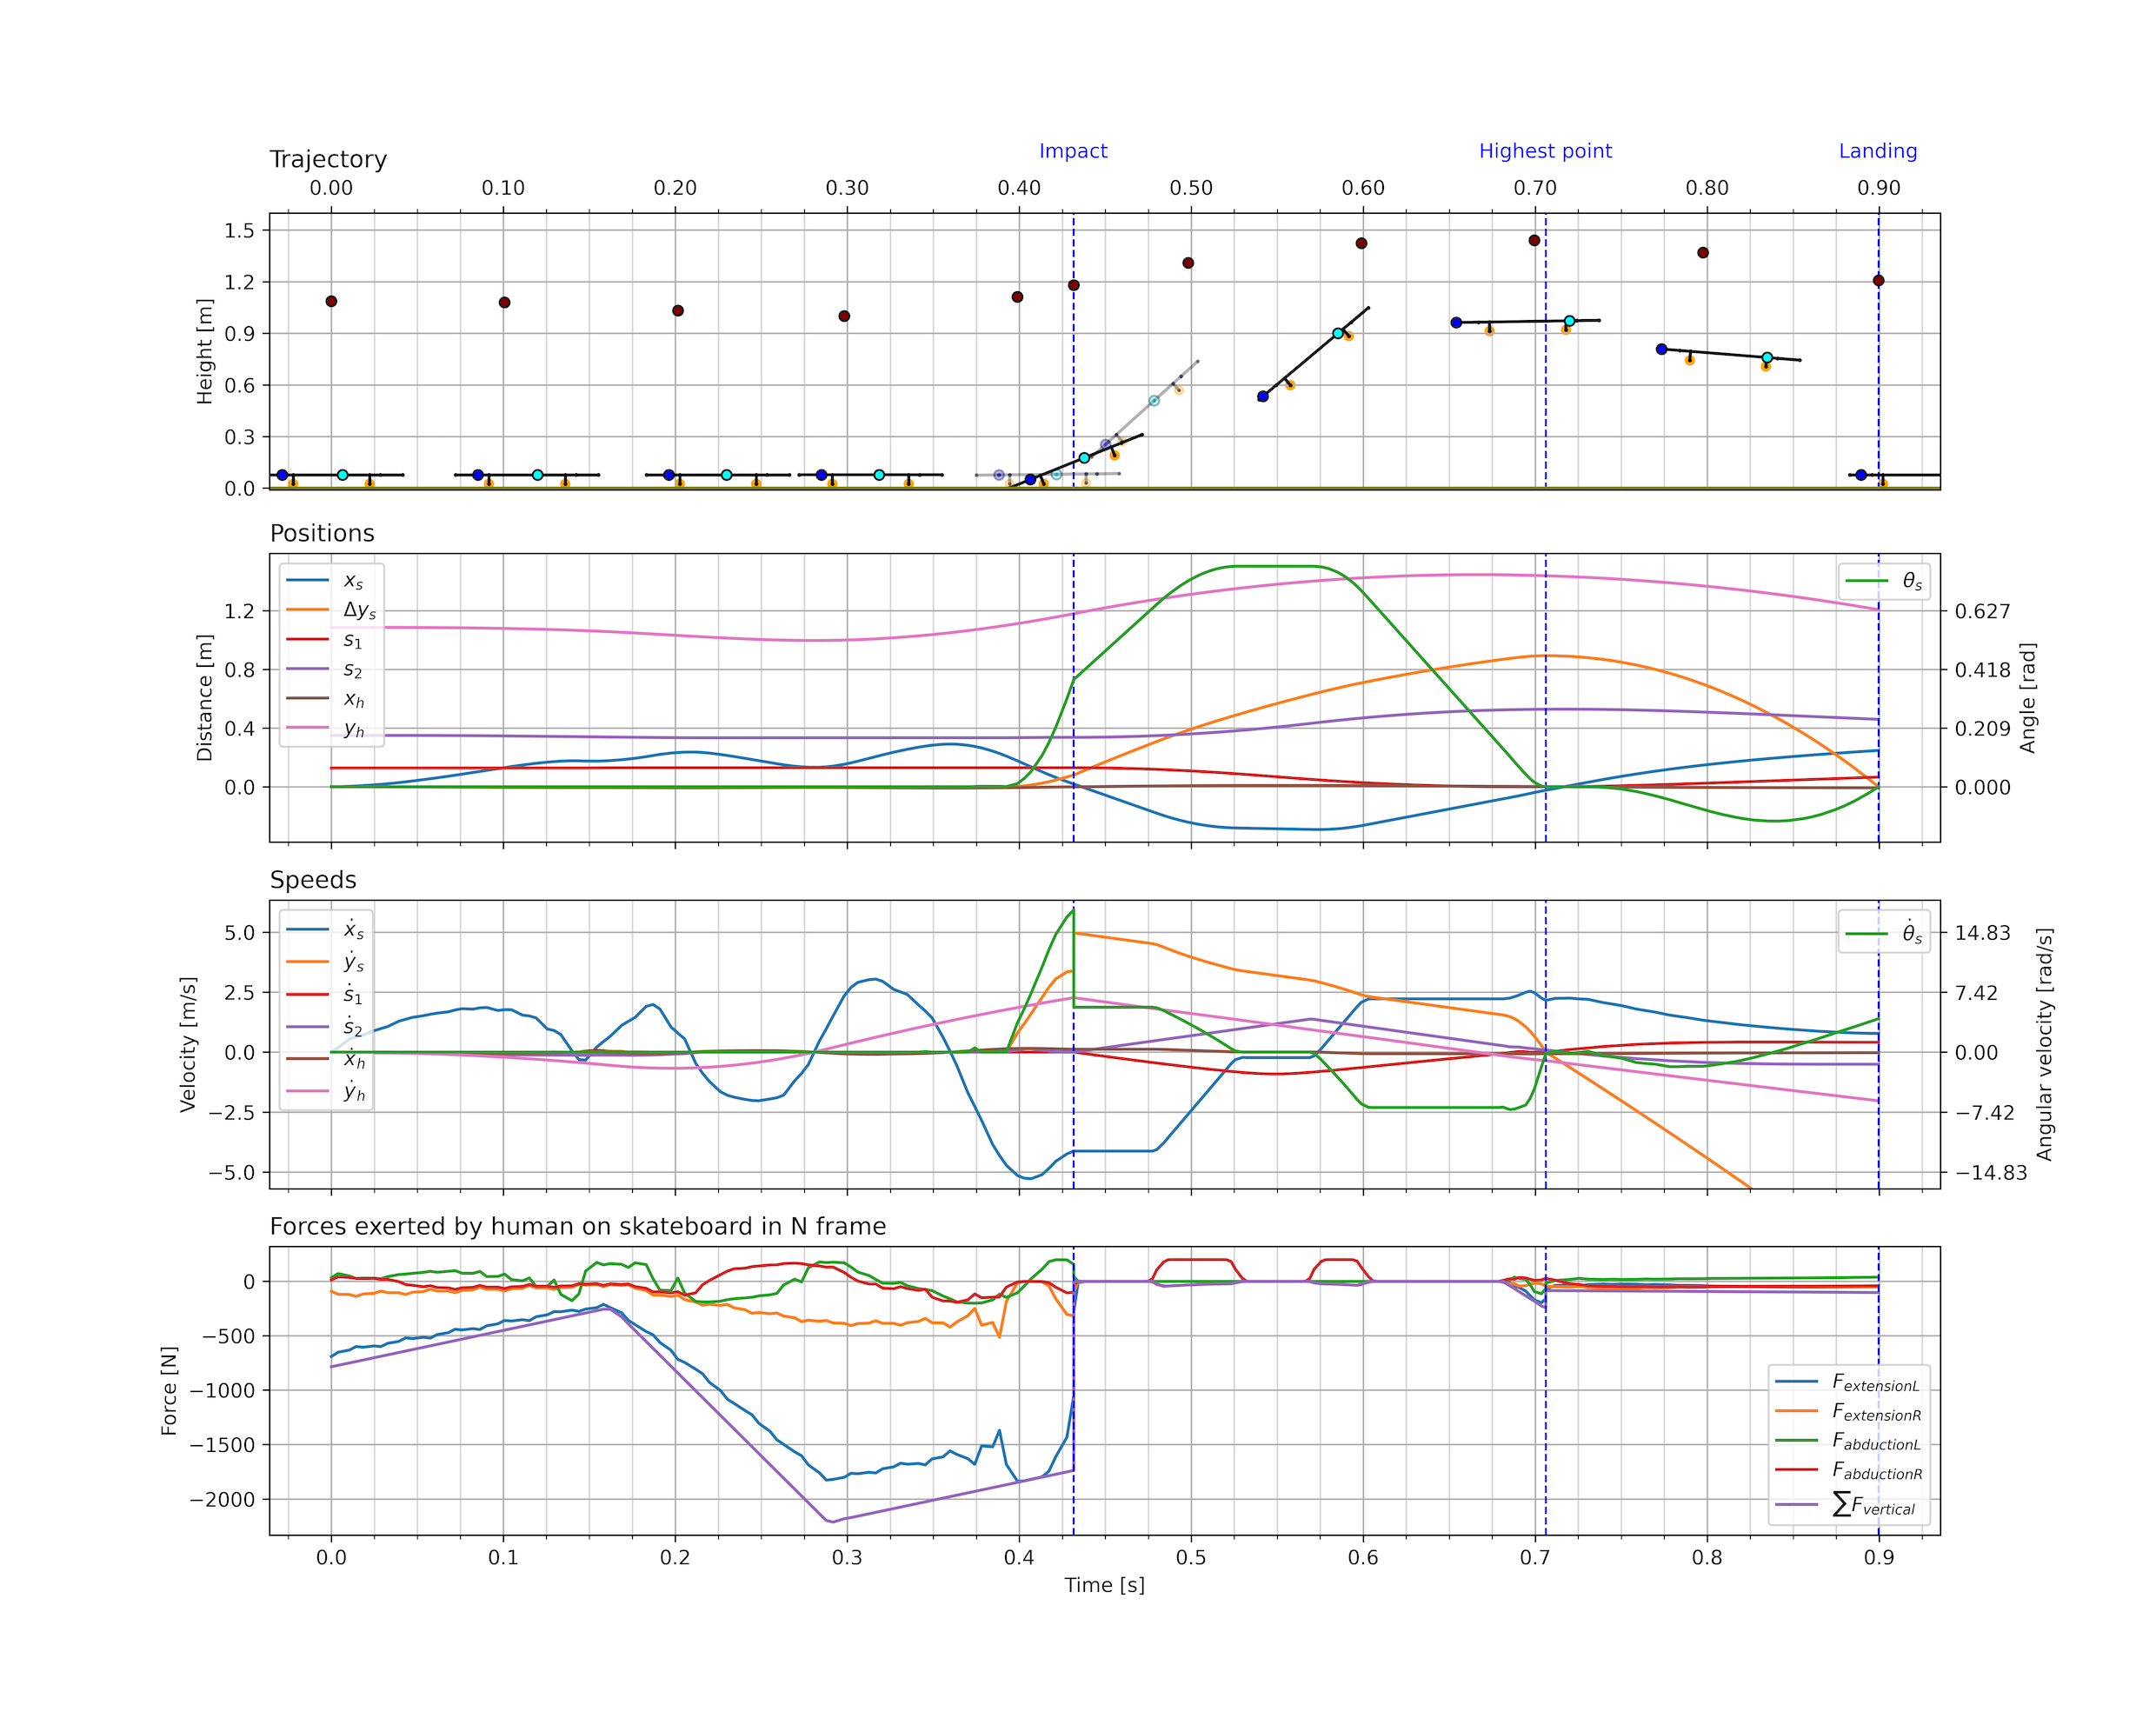
\includegraphics[trim={0cm 0cm 0cm 0cm},clip,width=0.8\textwidth]{figure/Results/data_phidpi600.png}}
    \newline
    \subfloat[All parameters]{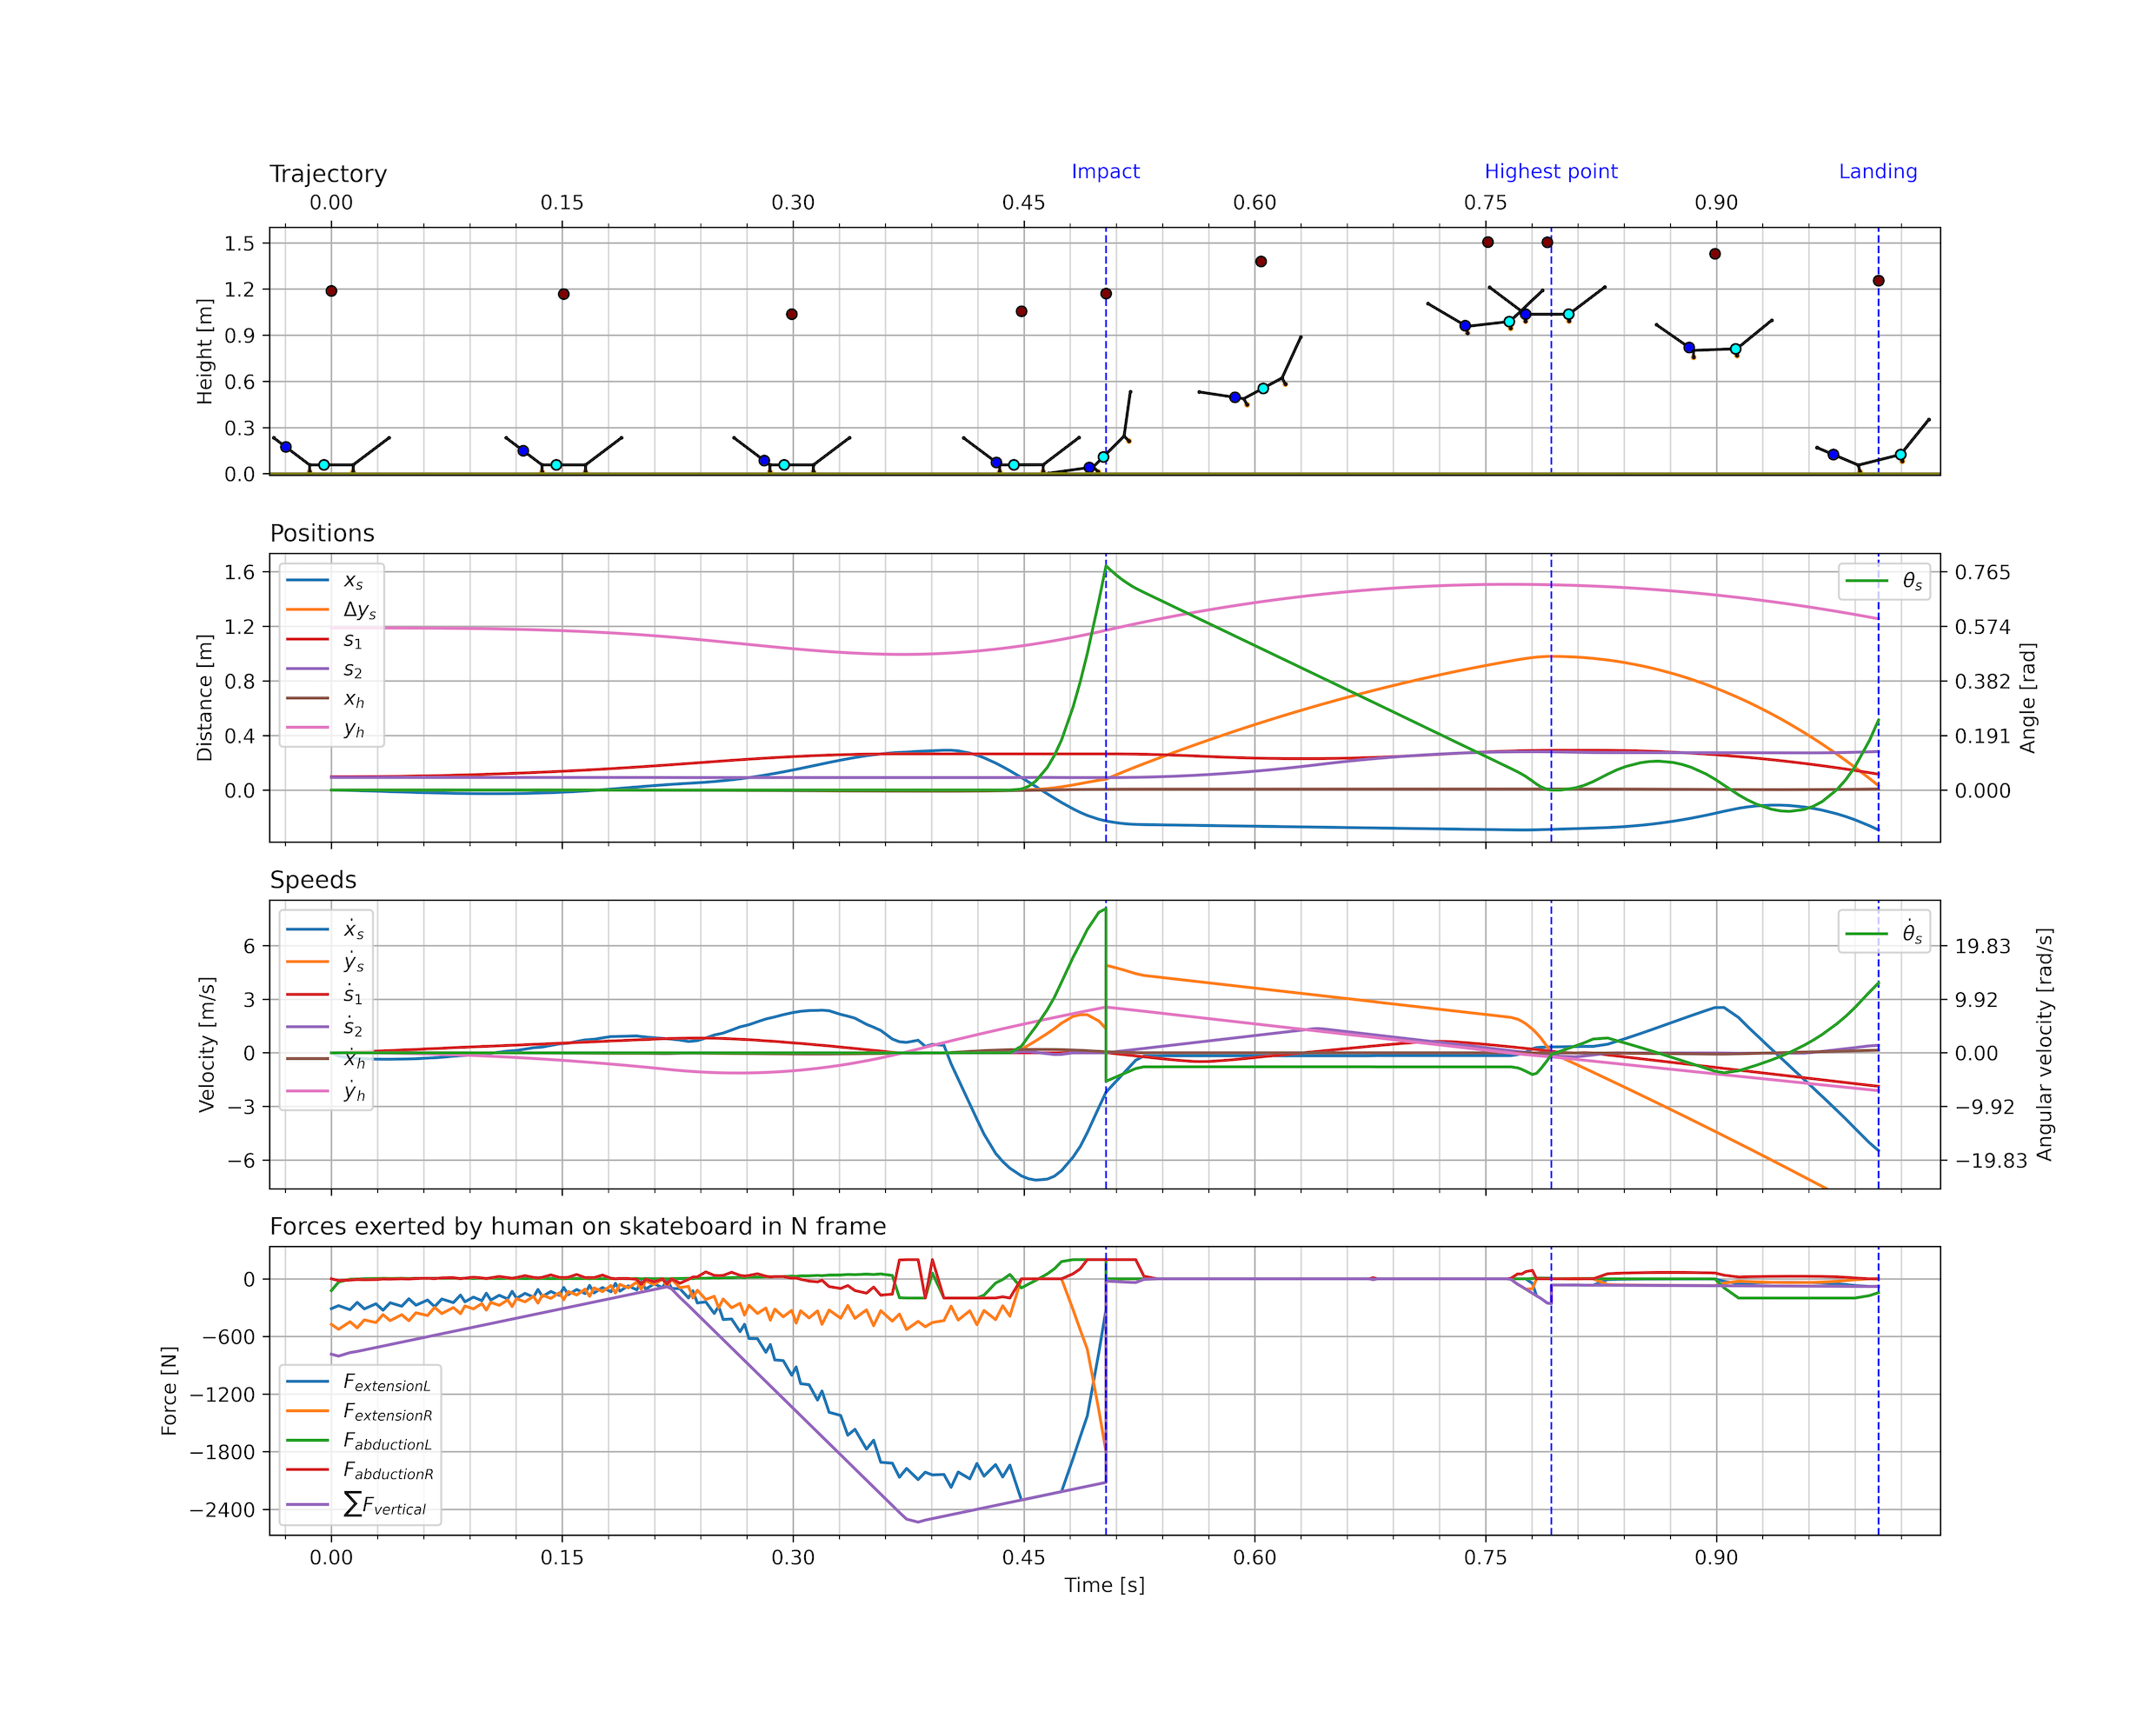
\includegraphics[trim={0cm 0cm 0cm 0cm},clip,width=0.8\textwidth]{figure/Results/data_alldpi600.png}}
    \caption{Tail inclination and all parameters optimization results}    
\end{figure*}


%Appendix will include inertia experiments and friction experiments

%% SHOW THAT NOSE ISN'T USED WHEN THE POSSIBILITY IS THERE

%% SHOW HOW VELOCITIES AFTER IMPACT ARE CALCULATED

%% SHOW 3 Friciton models
% During impact, friction can be present when there is a tangential velocity state relative to the impact surface. Poissons method and Newtons method have been shown unaccurate for such events and it is advised to use Stronge's method. This has been shown numerically in Stronge's comment on collision with friction\cite{stronge_comment_2010}. When the tail of the skateboard hits the ground, usually there is a tangential velocity state at the location of impact. This means that in real life a frictional impact occurs. Another implementation of the Poisson method during a frictional impact is solved with a set of constraints in the optimization\cite{patel_contact-implicit_2019}. The theory is that you create a variable $\phi(q_i)$, that represents the distance from the contact surface dependant on the generalized coordinates which should always be greater than 0. Furthermore there are three forces that should obey the friction cone presented in 